\documentclass[letterpaper,12pt]{report}
\usepackage[letterpaper,top=2.5cm,bottom=2.5cm,left=2.5cm,right=2.5cm]{geometry}
\usepackage[table]{xcolor}
\usepackage{graphicx,booktabs,amsmath,array,tabularx}
\usepackage{tikz}
\usetikzlibrary{positioning}
\usepackage{setspace}
\usepackage[unicode,hidelinks]{hyperref}
\usepackage{xepersian}
\settextfont[Path=fonts/,BoldFont=BNazaninBold.ttf]{BNazanin.ttf}
\setlatintextfont{FreeSerif}
\setdigitfont{FreeSerif}
\setlength{\parindent}{0.5cm}
\setlength{\parskip}{5pt}
\setlength{\emergencystretch}{2em}
\setstretch{1.3}
\setcounter{tocdepth}{2}
\renewcommand{\thesection}{\thechapter-\arabic{section}}
\renewcommand{\thesubsection}{\thesection-\arabic{subsection}}
\renewcommand{\thefigure}{\thechapter-\arabic{figure}}
\renewcommand{\thetable}{\thechapter-\arabic{table}}
\renewcommand{\bibname}{منابع}
\hypersetup{pdftitle={گزارش پروژه کارشناسی — نسخه تکمیل‌شده},pdfauthor={سید علی حسینی نسب}}
\begin{document}
\begin{titlepage}\centering
{\Large به نام خدا\par}
\vspace{0.6cm}

\includegraphics[width=2.8cm]{chapter3_assets/beheshti_logo.png}\par
\vspace{0.5cm}
{\Large دانشگاه شهید بهشتی\\[.2cm]دانشکده مهندسی و علوم کامپیوتر\par}
\vspace{1.1cm}
{\LARGE\bfseries تحلیل و تفسیر حرکات بازی شطرنج با استفاده از ترکیب موتورهای شطرنج و مدل‌های زبانی سبک\par}
\vspace{1cm}
{\Large پروژه کارشناسی\par}
\vspace{0.9cm}
{\large دانشجو:\\[.2cm]سید علی حسینی نسب\par}
\vspace{0.8cm}
{\large استاد راهنما:\\[.2cm]دکتر مهرنوش شمس فرد\par}
\vfill
\end{titlepage}
\chapter*{چکیده}\addcontentsline{toc}{chapter}{چکیده}
بازی شطرنج، به‌عنوان یکی از مسائل شناخته‌شده در حوزه هوش مصنوعی، با پیشرفت موتورهای شطرنجی به سطحی از دقت رسیده است که تحلیل تاکتیکی و ارزیابی موقعیت‌ها را با دقت بسیار بالا امکان‌پذیر می‌کند. با این حال، خروجی موتورهایی مانند \lr{Stockfish} معمولاً به‌صورت ارزیابی عددی و خطوط اصلی بازی ارائه می‌شود و برای بازیکنان، به‌ویژه بازیکنان مبتدی و متوسط، لزوماً قابل فهم و آموزشی نیست. از سوی دیگر، مدل‌های زبانی بزرگ توانایی بالایی در تولید متن روان دارند، اما در توضیح موقعیت‌های شطرنجی ممکن است دچار خطا یا ارائه تحلیل‌های نادرست شوند. هدف این پروژه، طراحی و پیاده‌سازی سامانه‌ای برای تولید توضیحات آموزشی و قابل فهم درباره حرکات شطرنج است که ضمن بهره‌گیری از توانایی تولید زبان طبیعی، به تحلیل دقیق موتور شطرنج نیز متکی باشد.

برای ارزیابی منصفانه و یکسان مدل‌ها، یک مجموعه‌داده آزمون متوازن شامل ۶۰نمونه از موقعیت‌ها و حرکات مختلف شطرنج از بازی‌های واقعی تهیه و به‌صورت دستی بررسی و برچسب‌گذاری شد. این مجموعه شامل ۲۰نمونه از هر یک از سطوح مبتدی، متوسط و پیشرفته است و برای هر نمونه، وضعیت صفحه قبل و بعد از حرکت، اطلاعات حرکت، تحلیل‌های مرتبط و یک توضیح مرجع آموزشی در نظر گرفته شده است. سپس ۱۱مدل زبانی با اندازه‌ها و قابلیت‌های متفاوت، از مدل کوچک مبتنی بر \lr{Qwen3-1.7B} با \lr{۱٫۷} میلیارد پارامتر تا مدل‌های جدیدتری مانند \lr{GPT-5.5} و \lr{Qwen3.7}بر روی این مجموعه آزمایش شدند. خروجی مدل‌ها نیز توسط یک مدل زبانی مستقل، \lr{Gemma 4 12B}، بر اساس معیارهایی شامل صحت، پیروی از دستور، مفیدبودن آموزشی، میزان انطباق با توضیح مرجع و روانی متن ارزیابی شد.

از نظر نرم‌افزاری، سامانه به‌صورت یک پایپالین چندمرحله‌ای طراحی شده است که در آن ابتدا اطلاعات موقعیت و حرکت شطرنج دریافت شده و با استفاده از \lr{Stockfish}تحلیل می‌شود؛ سپس ویژگی‌ها و تغییرات مهم صفحه توسط ماژول پردازش شطرنج استخراج شده و در قالب یک ورودی ساختاریافته به مدل زبانی داده می‌شود. این ساختار امکان آزمایش مدل‌های مختلف و مقایسه خروجی آن‌ها را در یک محیط یکسان فراهم می‌کند.

مدل اختصاصی مبتنی بر \lr{Qwen3-1.7B} با \lr{۱٫۷} میلیارد پارامتر، امتیاز کلی \lr{۲٫۸۶} از ده را کسب کرد. این امتیاز تقریباً برابر با مدل ۳ میلیاردپارامتری \lr{Llama 3.2} و نزدیک به \lr{Gemma 3 12B} با \lr{۲٫۹۵} و \lr{Gemma 4 26B A4B} با \lr{۲٫۹۰} است. بنابراین، مدل \lr{۱٫۷} میلیاردپارامتری در این مجموعه توانسته است میانگین امتیازی نزدیک به چند مدل بزرگ‌تر داشته باشد؛ هرچند این نتیجه به معنی برابری عمومی توانایی‌ها یا اثبات اثر آموزش دامنه نیست. بهترین مدل آزموده‌شده امتیاز \lr{۷٫۳۱} دارد و شکاف روانی و صحت در مدل کوچک همچنان باقی است. در مجموع، پروژه چارچوبی مشترک برای تولید و ارزیابی توضیحات شطرنجی فراهم می‌کند و ظرفیت مدل‌های سبک را در کنار ضرورت بهبود صحت محتوایی نشان می‌دهد.

واژگان کلیدی: هوش مصنوعی شطرنج، مدل‌های زبانی، تولید زبان طبیعی، ارزیابی مدل‌های زبانی، توضیح‌پذیری، تحلیل شطرنج
\clearpage
\begingroup
\setstretch{1.05}\setlength{\parskip}{0pt}
\tableofcontents\clearpage
\listoffigures\clearpage
\listoftables\clearpage
\endgroup
\chapter{کلیّات}

\section{مقدمه}

شطرنج یکی از محیط‌های مناسب برای مطالعه و ارزیابی سامانه‌های هوش مصنوعی به شمار می‌رود؛ زیرا هر موقعیت شطرنجی دارای ساختاری مشخص و قابل تحلیل است و کیفیت یک حرکت را می‌توان با استفاده از قواعد بازی و موتورهای تخصصی شطرنج بررسی کرد. در سال‌های اخیر، عالوه بر استفاده از موتورهای شطرنج برای تعیین بهترین حرکت، توجه به تولید توضیحات قابل فهم برای بازیکن نیز افزایش یافته است. در این رویکرد، هدف تنها مشخص کردن درست یا نادرست بودن یک حرکت نیست، بلکه لازم است دلیل مناسب بودن یا نبودن آن نیز به زبانی قابل درک برای کاربر بیان شود.

با ظهور مدل‌های زبانی، امکان استفاده از این مدل‌ها برای تولید توضیحات متنی درباره موقعیت‌های شطرنجی فراهم شده است. این مدل‌ها از نظر توانایی تولید متن و دنبال کردن دستورها عملکرد قابل توجهی دارند؛ بااین‌حال، تولید یک متن روان لزوماً به معنای صحیح بودن تحلیل شطرنجی آن نیست. یک مدل زبانی ممکن است توضیحی از نظر زبانی مناسب تولید کند، اما در آن ویژگی‌هایی از صفحه، تهدیدهای تاکتیکی یا پیامدهای واقعی یک حرکت را نادرست بیان نماید. بنابراین، یکی از چالش‌های اصلی در این حوزه، ارزیابی هم‌زمان کیفیت زبانی و صحت محتوای شطرنجی توضیحات تولید شده است.

از سوی دیگر، مقایسه مدل‌های زبانی مختلف برای یک مسئله یکسان، بدون وجود مجموعه آزمون و معیار ارزیابی مشترک، می‌تواند نتایج نامنظم و دشواری در مقایسه ایجاد کند. به همین دلیل، وجود یک مجموعه‌داده ارزیابی کنترل‌شده که شامل موقعیت‌های مختلف شطرنجی، سطوح متفاوت بازیکنان و توضیحات مرجع باشد، اهمیت زیادی دارد.

در این پروژه، یک سامانه نرم‌افزاری برای تولید و ارزیابی توضیحات شطرنجی طراحی شده است که در آن تحلیل موتور شطرنج با مدل‌های زبانی ترکیب می‌شود. همچنین یک مجموعه آزمون شامل  ۶۰نمونه از موقعیت‌ها و حرکات شطرنجی تهیه و برای مقایسه چندین مدل زبانی مورد استفاده قرار گرفته است. در نهایت، خروجی مدل‌ها با استفاده از یک مدل زبانی مستقل و بر اساس معیارهای مشخص ارزیابی شده است. هدف اصلی این فرایند، ایجاد روشی یکسان برای بررسی توانایی مدل‌های زبانی در تولید توضیحات صحیح و مفید درباره حرکات شطرنج است.

\section{بیان مسئله}

یکی از کاربردهای مهم سامانه‌های هوشمند شطرنج، کمک به بازیکن برای درک دلیل مناسب یا نامناسب بودن یک حرکت است. موتورهای شطرنجی مانند  \lr{Stockfish}می‌توانند موقعیت صفحه را با دقت بالا تحلیل کرده و حرکت‌های مناسب، تغییر ارزیابی موقعیت و خطوط اصلی بازی را مشخص کنند؛ اما خروجی چنین موتورهایی معمولاً به شکل عدد، حرکت پیشنهادی یا خط بازی ارائه می‌شود و لزوماً توضیح آموزشی و قابل فهمی برای یک بازیکن انسانی فراهم نمی‌کند.

این مسئله به‌خصوص برای بازیکنان مبتدی و متوسط اهمیت بیشتری دارد. بازیکن ممکن است بداند که یک حرکت باعث کاهش ارزیابی موقعیت شده است، اما برای یادگیری از اشتباه خود نیاز دارد بداند چرا این حرکت مشکل داشته است؛ برای مثال، آیا مهره‌ای بدون دفاع باقی مانده، ساختار پیاده‌ای ضعیف شده، امنیت شاه کاهش یافته یا یک فرصت تاکتیکی از دست رفته است.

بنابراین، تبدیل اطلاعات دقیق موتور شطرنج به توضیحی قابل فهم برای انسان، یک مسئله مهم در مسیر استفاده آموزشی از سامانه‌های هوشمند شطرنجی است.

مدل‌های زبانی می‌توانند برای حل این بخش از مسئله مورد استفاده قرار گیرند؛ زیرا توانایی تولید متن طبیعی و تبدیل اطلاعات ساختار یافته به توضیحات قابل فهم را دارند. بااین‌حال، استفاده مستقیم از مدل‌های زبانی با یک مشکل اساسی همراه است: توانایی تولید متن روان الزاماً ً نشان‌دهنده توانایی تحلیل صحیح موقعیت شطرنجی نیست. مدل ممکن است اطلاعاتی را تولید کند که از نظر زبانی منطقی به نظر برسد، اما با وضعیت واقعی صفحه یا تحلیل موتور شطرنج سازگار نباشد. این مسئله در ارزیابی مدل‌ها اهمیت زیادی دارد، زیرا مقایسه صرفاً بر اساس روان بودن متن نمی‌تواند کیفیت واقعی توضیحات شطرنجی را مشخص کند.

از طرف دیگر، مدل‌های زبانی موجود از نظر اندازه، معماری، قابلیت استدالل و هزینه اجرای محلی تفاوت قابل توجهی دارند. در نتیجه، انتخاب یک مدل مناسب برای تولید توضیحات شطرنجی نیازمند آزمایش مدل‌های مختلف بر روی ورودی‌ها و نمونه‌های یکسان است. در صورتی که مجموعه آزمون مناسبی وجود نداشته باشد، مقایسه مدل‌ها به‌شکل قابل اعتماد دشوار خواهد بود.

در این پروژه، مسئله اصلی به‌صورت زیر تعریف می‌شود:

چگونه می‌توان یک سامانه و فرایند ارزیابی طراحی کرد که در آن مدل‌های زبانی مختلف، با استفاده از اطلاعات واقعی و قابل بررسی شطرنجی، توضیحاتی درباره حرکات تولید کنند و این توضیحات بر اساس معیارهای یکسان از نظر صحت، مفید بودن و کیفیت زبانی با یکدیگر مقایسه شوند؟

برای پاسخ به این مسئله، لازم است چند چالش به‌صورت هم‌زمان مورد توجه قرار گیرد. نخست، نمونه‌های آزمون باید شامل موقعیت‌ها و حرکات متنوع باشند و سطوح مختلف بازیکنان را پوشش دهند. دوم، برای هر نمونه باید اطلاعات کافی از وضعیت قبل و بعد از حرکت و تحلیل شطرنجی آن وجود داشته باشد. سوم، برای مقایسه خروجی مدل‌ها به یک توضیح مرجع نیاز است که بتوان خروجی تولید شده را با آن مقایسه کرد. در نهایت، ارزیابی باید تا حد امکان مستقل از خود مدل تولیدکننده انجام شود.

بر این اساس، در این پروژه مجموعه‌ای متوازن شامل  ۶۰نمونه از بازی‌های واقعی شطرنج ایجاد شده که  ۲۰نمونه مربوط به هر یک از سطوح مبتدی، متوسط و پیشرفته است. برای هر نمونه، اطلاعات موقعیت قبل و بعد از حرکت، خود حرکت و اطلاعات تحلیلی مرتبط در نظر گرفته شده و توضیح مرجع آموزشی نیز تدوین شده است. سپس مدل‌های زبانی مختلف با استفاده از یک فرایند یکسان آزمایش شده و خروجی آن‌ها توسط یک مدل زبانی مستقل ارزیابی شده است.

وجه تمایز اصلی این پروژه در تمرکز هم‌زمان بر تولید توضیح، ایجاد مجموعه‌داده ارزیابی، مقایسه مدل‌های مختلف و ارزیابی مستقل خروجی‌ها است. همچنین در معماری پیشنهادی، اطلاعات حاصل از موتور شطرنج پیش از ارسال به مدل زبانی پردازش و به‌صورت ساختاریافته در اختیار آن قرار می‌گیرد تا مدل به جای تکیه صرف بر دانش زبانی خود، از شواهد قابل بررسی مربوط به موقعیت شطرنجی نیز استفاده کند.

\section{کلیات روش پیشنهادی}

هدف این پروژه، طراحی و پیاده‌سازی یک پایپالین نرم‌افزاری برای تحلیل موقعیت‌های شطرنج، تولید توضیحات زبانی و ارزیابی نظام‌مند مدل‌های زبانی است. روش پیشنهادی از دو پایپالین مرتبط تشکیل می‌شود. پایپالین نخست برای ساخت مجموعه آزمون مرجع و ارزیابی مدل‌های مختلف به کار می‌رود. پایپالین دوم نیز فرایند استفاده واقعی از سامانه را از زمان دریافت موقعیت یا حرکت از کاربر تا نمایش توضیح نهایی مدیریت می‌کند.

\subsubsection*{. ۱پایپالین ارزیابی مدل‌ها}

پایپالین ارزیابی مدل‌ها خود از دو فاز تشکیل شده است: فاز نخست به ساخت مجموعه آزمون مرجع اختصاص دارد و در فاز دوم، مدل‌های زبانی با استفاده از این مجموعه آزمایش و مقایسه می‌شوند.

\subsubsection*{فاز اول: ساخت مجموعه آزمون مرجع}

در نخستین مرحله، بازی‌های واقعی شطرنج بررسی شد و از میان آن‌ها  ۶۰حرکت یا موقعیت برای تشکیل مجموعه آزمون انتخاب شد. نمونه‌ها به‌گونه‌ای انتخاب و دسته‌بندی شد که بازیکنان با سطوح مهارتی مختلف و انواع متنوعی از حرکات، اشتباهات و موقعیت‌های تاکتیکی و استراتژیک در مجموعه حضور داشته باشند. برای هر نمونه، اطلاعاتی مانند وضعیت صفحه پیش از حرکت، حرکت انجام‌شده، وضعیت صفحه پس از حرکت و سایر داده‌های لازم ذخیره شد.

در مرحله بعد، وضعیت صفحه پیش و پس از هر حرکت با استفاده از موتور شطرنج  \lr{Stockfish}تحلیل شد. این تحلیل شامل امتیاز موقعیت، بهترین حرکت پیشنهادی، خطوط اصلی بازی، تغییر امتیاز پس از حرکت و میزان فاصله حرکت بازیکن با انتخاب پیشنهادی موتور است.

پس از دریافت تحلیل، \lr{Stockfish}اطلاعات مربوط به دو وضعیت قبل و بعد از حرکت با یکدیگر مقایسه شدند. در این مرحله، ویژگی‌های مهم شطرنجی مانند تغییر ارزیابی موقعیت، جابه‌جایی یا از دست رفتن مهره‌ها، ساختار پیاده‌ای، امنیت شاه، کنترل خانه‌های مهم، تهدیدهای ایجاد شده و برخی الگوهای تاکتیکی و موقعیتی استخراج می‌شوند.

سپس هر یک از  ۶۰نمونه به‌صورت انسانی بررسی و برچسب‌گذاری می‌شود. برای هر موقعیت، یک پاسخ مرجع شامل توضیح مناسب درباره حرکت، پیامدهای آن و دلایل احتمالی خوب یا نامناسب بودن حرکت تهیه می‌شود. در پایان این فاز، مجموعه آزمون مرجع شامل داده‌های شطرنجی، نتایج تحلیل، \lr{Stockfish}ویژگی‌های استخراج‌شده و توضیح انسانی آماده خواهد بود.

\subsubsection*{فاز دوم: آزمون و مقایسه مدل‌ها}

پس از آماده‌شدن مجموعه آزمون مرجع، مدل زبانی مورد ارزیابی روی همان  ۶۰نمونه اجرا می‌شود. برای هر نمونه، اطلاعات حاصل از  \lr{Stockfish}و ماژول استخراج ویژگی در قالب یک ورودی ساختاریافته در اختیار مدل قرار

می‌گیرد. این ورودی می‌تواند شامل وضعیت صفحه، حرکت بازیکن، تغییر امتیاز، بهترین حرکت پیشنهادی موتور و ویژگی‌های تاکتیکی و موقعیتی استخراج‌شده باشد.

مدل مورد آزمایش با استفاده از این اطلاعات، توضیحی متنی درباره حرکت تولید می‌کند. خروجی‌های مدل در قالبی مشخص دریافت، ذخیره و یکسان‌سازی می‌شوند تا تفاوت‌های ظاهری یا ساختاری مانع ارزیابی منصفانه مدل‌ها نشوند. این فرایند برای تمام نمونه‌های مجموعه آزمون و برای هر مدل زبانی مورد بررسی تکرار می‌شود.

در مرحله ارزیابی، توضیح تولید شده توسط هر مدل با پاسخ انسانی مرجع همان نمونه مقایسه می‌شود. برای انجام این مقایسه، مدل مستقل  \lr{Gemma 4 12B}به‌عنوان داور به کار می‌رود. این مدل بر اساس معیارهای از پیش تعیین‌شده، میزان تطابق پاسخ مدل با پاسخ مرجع را بررسی می‌کند. معیارهای ارزیابی می‌توانند شامل صحت شطرنجی، ارتباط توضیح با حرکت، پوشش نکات اصلی، نبود ادعاهای نادرست، وضوح متن و میزان شباهت محتوایی به پاسخ مرجع باشند.

در پایان، خطاها و امتیازهای هر مدل محاسبه می‌شوند. نتایج به‌صورت تجمیعی و در سطح هر نمونه ذخیره می‌شوند تا مقایسه مدل‌ها، شناسایی نقاط ضعف آن‌ها و انتخاب مناسب‌ترین مدل برای استفاده در سامانه امکان‌پذیر باشد.

\subsubsection*{. ۲پایپالین استفاده واقعی}

پایپالین دوم مربوط به زمانی است که کاربر از سامانه استفاده می‌کند. در این حالت، کاربر یک حرکت یا موقعیت شطرنجی را وارد می‌کند. ورودی می‌تواند شامل وضعیت صفحه و حرکت انجام‌شده یا وضعیت صفحه پیش و پس از حرکت باشد.

این اطلاعات ابتدا برای تحلیل به  \lr{Stockfish}ارسال می‌شوند. موتور شطرنج وضعیت موجود، کیفیت حرکت، بهترین ادامه‌های ممکن و تغییر ارزیابی ناشی از حرکت را مشخص می‌کند. سپس خروجی موتور وارد ماژول پردازش شطرنج می‌شود.

ماژول پردازش، خروجی  \lr{Stockfish}و اطلاعات صفحه را بررسی می‌کند و با استفاده از قواعد اکتشافی، ویژگی‌های قابل توضیح را استخراج می‌کند. این قواعد می‌توانند برای تشخیص مواردی مانند از دست رفتن مهره، ایجاد تهدید، ضعف امنیت شاه، تغییر ساختار پیاده‌ای، کنترل خطوط باز یا شکل‌گیری یک الگوی تاکتیکی استفاده شوند.

داده‌های حاصل در قالب یک ورودی ساختاریافته به مدل زبانی منتخب ارسال می‌شوند. این مدل همان مدلی است که بر اساس نتایج پایپالین ارزیابی، عملکرد مناسب‌تری داشته است. مدل زبانی با تکیه بر اطلاعات ارائه‌شده، توضیحی قابل‌فهم درباره حرکت تولید می‌کند و متن نهایی از طریق رابط کاربری به کاربر نمایش داده می‌شود.

\subsubsection*{معماری نرم‌افزاری سامانه}

معماری کلی نرم‌افزار شامل موتور تحلیل شطرنج، ماژول استخراج ویژگی و قواعد اکتشافی، بخش ساخت ورودی، ماژول ارتباط با مدل‌های زبانی، پایگاه ذخیره نتایج \lr{Backend}، برای مدیریت پردازش‌ها و \lr{API}ها و  \lr{Frontend}برای تعامل کاربر با سامانه است.

تفکیک این بخش‌ها باعث می‌شود مدل زبانی، موتور شطرنج یا معیارهای ارزیابی بدون ایجاد تغییر اساسی در کل سامانه جایگزین یا اصلاح شوند. همچنین می‌توان مدل‌های مختلف را با ورودی‌ها، تنظیمات و معیارهای یکسان آزمایش کرد و نتایج آن‌ها را در شرایط قابل‌مقایسه به دست آورد.

روند کلی روش پیشنهادی در شکل~\ref{fig:intro-flow} نمایش داده شده است.
\begin{figure}[htbp]\centering
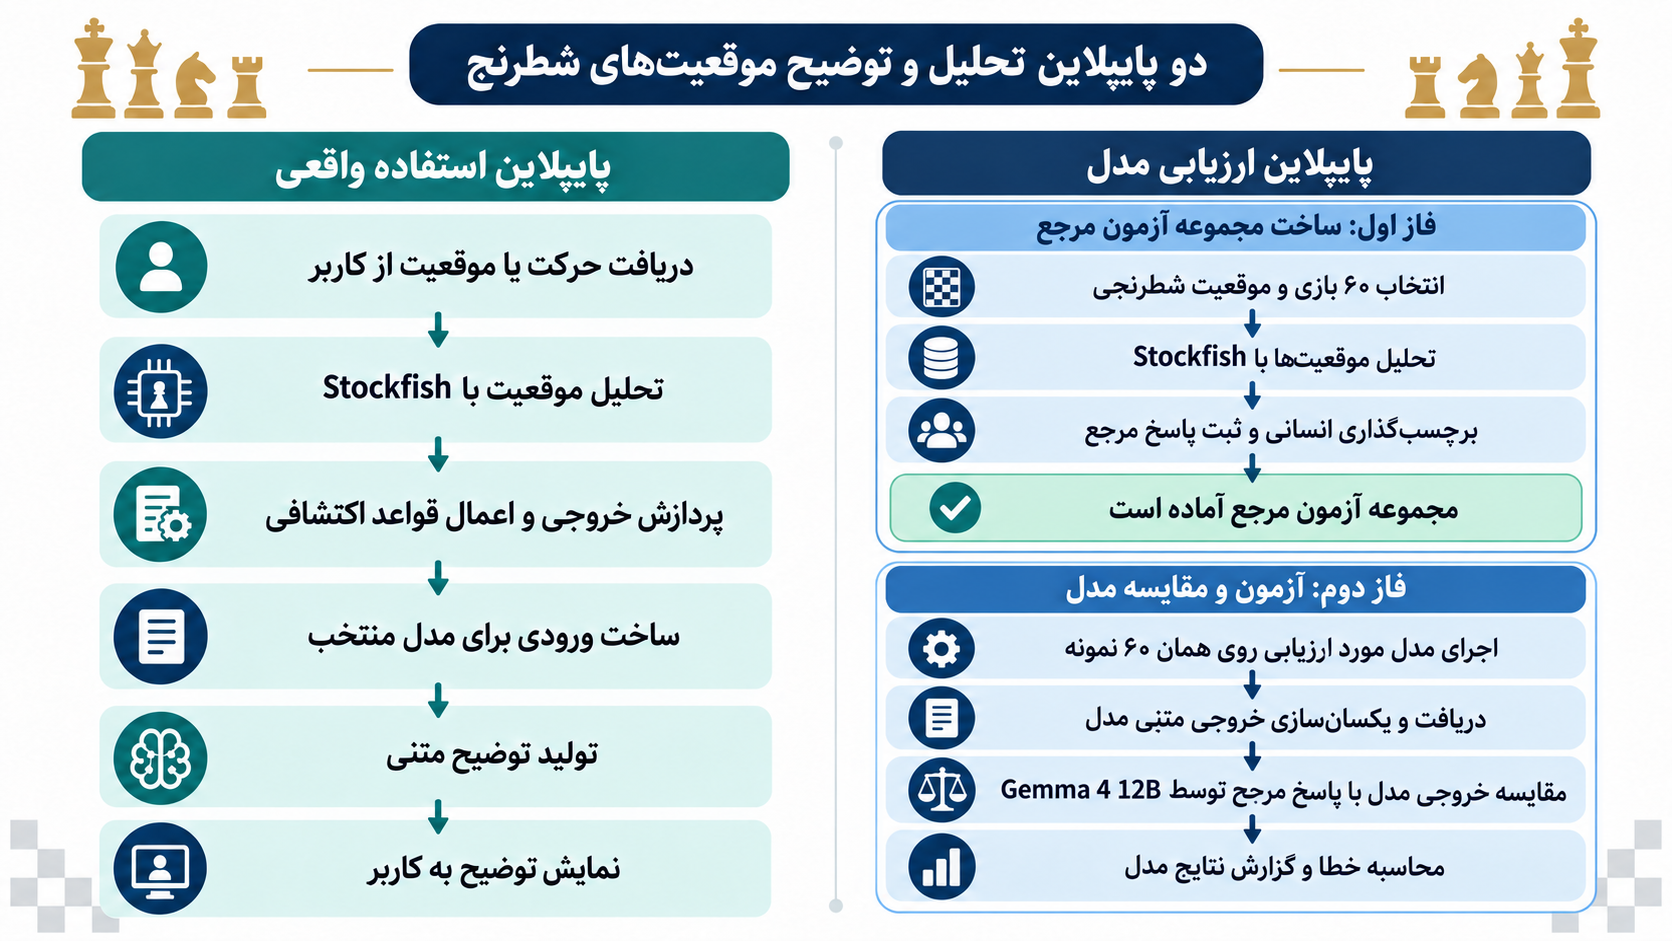
\includegraphics[width=\linewidth]{chapter3_assets/original_intro.png}
\caption{روند کلی ساخت، ارزیابی و استفاده از سامانه}\label{fig:intro-flow}
\end{figure}

بنابراین، خروجی نهایی پروژه صرفاً یک مدل تولیدکننده توضیحات شطرنجی نیست، بلکه یک سامانه نرم‌افزاری و چارچوب آزمایشی یکپارچه است. این سامانه از یک سو موقعیت‌های شطرنج را تحلیل کرده و توضیح قابل‌فهمی در اختیار کاربر قرار می‌دهد و از سوی دیگر، امکان آزمایش، ارزیابی و مقایسه مدل‌های زبانی مختلف را با استفاده از یک مجموعه آزمون مرجع فراهم می‌کند.

\section{ساختار پروژه}

این گزارش در سه فصل اصلی تنظیم شده است. در فصل اول، کلیات پروژه شامل مقدمه، بیان مسئله، هدف و روش پیشنهادی و همچنین ساختار گزارش ارائه می‌شود.

در فصل دوم، مفاهیم و فناوری‌های مرتبط با پروژه بررسی می‌شوند. در این فصل ابتدا مفاهیم پایه مرتبط با تحلیل شطرنج، موتورهای شطرنج، مدل‌های زبانی و تولید توضیحات متنی معرفی شده و سپس پژوهش‌ها و سامانه‌های مشابه مورد بررسی و مقایسه قرار می‌گیرند. هدف این فصل، مشخص کردن جایگاه پروژه حاضر در میان روش‌ها و سامانه‌های موجود است.

در فصل سوم، روش پیشنهادی و جزئیات پیاده‌سازی ارائه می‌شود. ساختار سامانه، اجزای مختلف پایپالین نرم‌افزاری، نحوه ایجاد مجموعه آزمون، فرایند تحلیل موقعیت‌ها، نحوه استفاده از مدل‌های زبانی و روش ارزیابی خروجی‌ها در این فصل تشریح می‌شوند. در ادامه نیز نتایج حاصل از آزمایش مدل‌های مختلف ارائه و تحلیل خواهند شد.

در پایان گزارش، منابع مورد استفاده در تهیه و انجام پروژه مطابق قالب استاندارد ارائه می‌شوند.

\chapter{مفاهیم پایه و کارهای مرتبط}

\section{مقدمه}

در این فصل، مفاهیم و پژوهش‌های مرتبط با تولید و ارزیابی توضیحات شطرنجی مبتنی بر مدل‌های زبانی بررسی می‌شوند. مسئله مورد بررسی در این پروژه در نقطه تلاقی چند حوزه قرار دارد: تحلیل شطرنج توسط موتورهای تخصصی، مدل‌های زبانی و تولید زبان طبیعی، تولید توضیحات برای تصمیمات پیچیده و ارزیابی کیفیت خروجی مدل‌های زبانی. بنابراین، برای درک روش پیشنهادی، لازم است ابتدا ارتباط میان این مفاهیم مشخص شود.

در ساده‌ترین حالت، می‌توان فرایند مورد نظر را به این صورت در نظر گرفت که یک موقعیت شطرنجی به‌عنوان ورودی دریافت می‌شود و یک موتور شطرنج با بررسی وضعیت صفحه، اطلاعاتی درباره کیفیت حرکت و تغییرات موقعیت ارائه می‌کند. این اطلاعات در مرحله بعد می‌تواند به یک مدل زبانی داده شود تا آن را به توضیحی قابل فهم برای انسان تبدیل کند. در نهایت، توضیح تولید شده باید با استفاده از معیارهای مشخص ارزیابی شود. بنابراین، موتور شطرنج نقش تأمین اطلاعات تخصصی و قابل بررسی را دارد، مدل زبانی وظیفه تبدیل این اطلاعات به زبان طبیعی را بر عهده می‌گیرد و بخش ارزیابی کیفیت خروجی را بررسی می‌کند.

یکی از دلایل اهمیت این زنجیره آن است که هر بخش محدودیت‌های خاص خود را دارد. موتورهای شطرنج در ارزیابی موقعیت و انتخاب حرکت بسیار قدرتمند هستند، اما خروجی آن‌ها معمولاً به‌صورت عددی یا در قالب خطوط بازی ارائه می‌شود و برای آموزش مستقیم انسان مناسب نیست. در مقابل، مدل‌های زبانی در تولید متن روان و قابل فهم توانایی بالایی دارند، اما ممکن است در توضیح موقعیت‌های تخصصی، اطلاعات نادرست تولید کنند. پژوهش‌های جدید نیز این فاصله میان دقت مدل‌های تخصصی و قابلیت توضیح‌دهی مدل‌های زبانی را به‌عنوان یکی از چالش‌های اصلی این حوزه مطرح کرده‌اند.

\subsection{تحلیل شطرنج و موتورهای شطرنج}

موتور شطرنج نرم‌افزاری است که با بررسی وضعیت صفحه و جست‌وجوی حرکت‌های ممکن، تالش می‌کند بهترین تصمیم را برای یک موقعیت مشخص پیدا کند. خروجی موتور می‌تواند شامل حرکت پیشنهادی، ارزیابی موقعیت و خطوط احتمالی ادامه بازی باشد. در پروژه حاضر، موتور  \lr{Stockfish}به‌عنوان منبع تحلیل تخصصی مورد استفاده قرار می‌گیرد.

اهمیت موتور شطرنج در این پروژه تنها در پیدا کردن بهترین حرکت نیست. اطلاعات موتور به‌عنوان یک مبنای قابل بررسی برای تشخیص تغییرات ایجادشده در نتیجه یک حرکت نیز استفاده می‌شود. به این ترتیب، مدل زبانی می‌تواند به جای تولید توضیح صرفاً بر اساس الگوهای زبانی، از اطلاعات حاصل از تحلیل موقعیت نیز استفاده کند.

این ایده با برخی پژوهش‌های پیشین نیز هم‌راستا است. برای نمونه \lr{Lee}، و همکاران نشان داده‌اند که ترکیب مدل‌های زبانی با موتورهای استدالل نمادین می‌تواند برای تولید توضیحات شطرنجی مفید باشد و این ترکیب، امکان استفاده هم‌زمان از توانایی تحلیلی موتور و توانایی زبانی مدل را فراهم می‌کند.

\subsection{مدل‌های زبانی و تولید متن}

مدل زبانی، مدلی یادگیری‌محور است که با استفاده از الگوهای موجود در داده‌های متنی می‌تواند متن تولید کند، دستورها را دنبال کند و اطلاعات ورودی را به زبان طبیعی بازنمایی کند. مدل‌های زبانی جدید در بسیاری از وظایف تولید متن عملکرد قابل توجهی دارند و می‌توانند برای تبدیل داده‌های ساختاریافته به توضیحات قابل فهم استفاده شوند.

در مسئله شطرنج، استفاده از مدل زبانی به این دلیل اهمیت دارد که خروجی موتور شطرنج برای بسیاری از کاربران، به‌خصوص بازیکنان مبتدی، مستقیما ً قابل تفسیر نیست. برای مثال، دانستن اینکه ارزیابی یک موقعیت پس از یک حرکت کاهش یافته است، به‌تنهایی توضیح نمی‌دهد که این کاهش به دلیل ضعف امنیت شاه، از دست دادن یک مهره، ایجاد ضعف در ساختار پیاده‌ها یا از دست دادن یک فرصت تاکتیکی رخ داده است.

با این حال، مدل زبانی به‌تنهایی تضمین نمی‌کند که توضیح تولید شده از نظر شطرنجی صحیح باشد. پژوهش‌های مرتبط نشان داده‌اند که مدل‌های زبانی می‌توانند توضیحاتی روان تولید کنند، در حالی که برخی ادعاهای موجود در آن‌ها با وضعیت واقعی صفحه سازگار نیست. به همین دلیل، استفاده از اطلاعات موتور شطرنج و روش‌های ارزیابی مستقل اهمیت پیدا می‌کند.

\subsection{تولید توضیحات شطرنجی}

تولید توضیحات شطرنجی را می‌توان به‌عنوان مسئله‌ای برای تبدیل اطلاعات یک بازی یا موقعیت شطرنجی به متن طبیعی تعریف کرد. در پژوهش  \lr{Jhamtani}~\cite{jhamtani2018}و همکاران، این مسئله با استفاده از مجموعه‌داده بزرگی شامل بیش از  ۲۹۸هزار جفت حرکت و توضیح در بیش از  ۱۱هزار بازی بررسی شده است. این پژوهش نشان می‌دهد که توضیح دادن حرکات شطرنجی تنها به وضعیت فعلی صفحه وابسته نیست و ویژگی‌های مختلف بازی و زمینه حرکت نیز می‌توانند در نوع توضیح تولیدشده مؤثر باشند.

در پژوهش  \lr{Zang}~\cite{zang2019}و همکاران نیز تولید خودکار توضیحات شطرنجی در دسته‌هایی مانند توصیف، مقایسه و برنامه‌ریزی بررسی شده است. این پژوهش با وارد کردن یک موتور شطرنج عصبی در مدل تولید متن، تالش می‌کند اطلاعات مربوط به صفحه و تصمیم شطرنجی را با فرایند تولید زبان طبیعی ترکیب کند. ارزیابی این روش نیز هم با معیارهای خودکار و هم با ارزیابی انسانی انجام شده است.

این مطالعات نشان می‌دهند که تولید توضیح شطرنجی یک مسئله صرفاً زبانی نیست و برای تولید توضیح مناسب، درک وضعیت صفحه و تصمیم اتخاذشده نیز اهمیت دارد.

\subsection{اتصال تحلیل تخصصی و مدل زبانی}

یکی از رویکردهای مهم در پژوهش‌های جدید، ترکیب یک سامانه تخصصی با مدل زبانی است. در این رویکرد، سامانه تخصصی اطلاعات دقیق مربوط به مسئله را فراهم می‌کند و مدل زبانی وظیفه تبدیل آن اطلاعات به یک خروجی قابل فهم را بر عهده می‌گیرد.

دکتر  \lr{Kim}~\cite{kim2025}و همکاران در سال  ۲۰۲۵با معرفی روش \lr{Concept-guided Chess Commentary Generation}تالش کردند توانایی تصمیم‌گیری مدل‌های تخصصی را با قابلیت تولید زبان طبیعی مدل‌های زبانی ترکیب کنند. در این روش، توضیحات بر اساس مفاهیم شطرنجی هدایت می‌شوند و در کنار روش تولید، یک روش ارزیابی مبتنی بر دانش تخصصی نیز معرفی شده است. نتایج این پژوهش با ارزیابی انسانی و ارزیابی مبتنی بر مدل زبانی بررسی شده‌اند.

این رویکرد به مسئله پروژه حاضر نزدیک است؛ زیرا در هر دو، هدف آن است که اطلاعات تخصصی شطرنج به توضیح قابل فهم تبدیل شود. تفاوت مهم پروژه حاضر در تمرکز آن بر ایجاد یک مجموعه آزمون متوازن، مقایسه تعداد زیادی مدل زبانی مختلف و ارزیابی خروجی آن‌ها در یک فرایند یکسان است.

\subsection{ارزیابی توضیحات شطرنجی}

یکی از چالش‌های مهم این حوزه، تعیین کیفیت توضیح تولید شده است. ارزیابی یک متن شطرنجی تنها بر اساس روان بودن آن کافی نیست؛ زیرا ممکن است متن از نظر زبانی مناسب باشد اما ادعاهای شطرنجی نادرستی داشته باشد.

پژوهش‌های اولیه از ارزیابی انسانی و معیارهای خودکار برای بررسی کیفیت توضیحات استفاده کرده‌اند. برای مثال، \lr{Jhamtani}~\cite{jhamtani2018}و همکاران عالوه بر مقایسه مدل‌ها، بخشی از خروجی‌ها را توسط انسان‌ها از نظر صحت و روانی بررسی کردند.

در پژوهش  \lr{Kim}~\cite{kim2025}و همکاران نیز عالوه بر تولید توضیح، یک چارچوب ارزیابی مبتنی بر مدل زبانی و دانش تخصصی معرفی شده است. این موضوع نشان می‌دهد که مسئله ارزیابی توضیحات به اندازه مسئله تولید آن اهمیت دارد.

پژوهش جدیدتر  \lr{Hebbar}~\cite{hebbar2026}و همکاران در سال  ۲۰۲۶این مسئله را با تمرکز مستقیم بر توهم در توضیحات شطرنجی بررسی می‌کند. در این پژوهش، چارچوب  \lr{ACT-Eval}ادعاهای موجود در توضیحات را به اجزای کوچک‌تر تقسیم کرده و آن‌ها را با استفاده از ابزارهای مبتنی بر موتور و مراجع تأییدشده بررسی می‌کند. این پژوهش همچنین یک بنچمارک شامل  ۳۲۵جفت موقعیت-حرکت ارائه می‌دهد و نشان می‌دهد که خطاهای محتوایی در توضیحات مدل‌های زبانی همچنان مسئله‌ای جدی هستند.

پژوهش  \lr{Cui}~\cite{cui2026}و همکاران نیز به‌طور مستقیم مسئله بیان استراتژی‌های شطرنج در زبان طبیعی را بررسی کرده و عالوه بر روش تولید توضیح، یک چارچوب برای ارزیابی عینی توضیحات پیشنهاد می‌کند. این پژوهش همچنین محدودیت ارزیابی صرفاً مبتنی بر مدل‌های زبانی را مورد توجه قرار می‌دهد.

در نتیجه، در پروژه حاضر نیز ارزیابی خروجی‌ها به‌عنوان یکی از اجزای اصلی در نظر گرفته می‌شود. برای این منظور، خروجی مدل‌های مختلف با استفاده از معیارهای یکسان و توسط یک مدل ارزیاب مستقل بررسی می‌شوند.

\section{تحلیل نقاط قوت و ضعف منابع غیرپژوهشی مشابه}

در کنار پژوهش‌های دانشگاهی، برخی سامانه‌های تجاری و عمومی شطرنج نیز قابلیت‌هایی برای توضیح متنی حرکات و موقعیت‌های شطرنجی ارائه می‌کنند. هدف اصلی این سامانه‌ها معمولاً تحلیل و آموزش شطرنج برای کاربران است و نه بررسی و مقایسه مدل‌های زبانی. بااین‌حال، از آنجا که برخی از این سامانه‌ها برای حرکات شطرنجی توضیحات متنی تولید می‌کنند، می‌توان آن‌ها را از نظر قابلیت‌های ارائه‌شده و تفاوت با سامانه پیشنهادی این پروژه بررسی کرد.

یکی از نقاط قوت این سامانه‌ها، ارائه یک محیط یکپارچه و آماده استفاده برای کاربر است. کاربر می‌تواند موقعیت یا بازی شطرنجی خود را در اختیار سامانه قرار دهد، تحلیل شطرنج را مشاهده کند و در برخی موارد، عالوه بر اطلاعات مربوط به حرکت، یک توضیح متنی نیز دریافت کند. این موضوع باعث می‌شود استفاده از قابلیت‌های تحلیلی برای کاربران، به‌ویژه کاربران غیرمتخصص، ساده‌تر شود.

بااین‌حال، نحوه تولید توضیحات متنی در بسیاری از این سامانه‌ها برای کاربر قابل مشاهده نیست. به‌طور مشخص، مشخص نیست که متن تولیدشده دقیقاً توسط چه مدل یا ترکیبی از چه روش‌هایی ایجاد می‌شود و چه اطلاعاتی از وضعیت شطرنج برای تولید آن در اختیار سامانه قرار می‌گیرد. در نتیجه، امکان بررسی دقیق ارتباط میان تحلیل شطرنج، اطلاعات ورودی و متن نهایی تولیدشده برای یک کاربر یا پژوهشگر وجود ندارد.

محدودیت دیگر، وابستگی این قابلیت‌ها به سرویس‌های آنالین است. توضیحات متنی در این سامانه‌ها معمولاً در سمت سرور تولید می‌شوند و کاربر تنها نتیجه نهایی را دریافت می‌کند. بنابراین، مدل یا فرایند تولیدکننده متن لزوماً به‌صورت محلی در اختیار کاربر قرار نمی‌گیرد. این مسئله با هدف پروژه حاضر که بررسی امکان استفاده از مدل‌های زبانی به‌صورت محلی و قابل کنترل است، تفاوت دارد.

از طرف دیگر، این سامانه‌ها برای مقایسه چند مدل زبانی مختلف نیز طراحی نشده‌اند. در پروژه حاضر، هدف آن است که مدل‌های مختلف با ورودی یکسان روی یک مجموعه آزمون مشخص آزمایش شوند و خروجی آن‌ها با استفاده از معیارهای یکسان مورد ارزیابی قرار گیرد. به همین دلیل، تمرکز پروژه حاضر نه بر رقابت با امکانات عمومی سامانه‌های شطرنجی، بلکه بر فراهم کردن یک محیط قابل بررسی برای مطالعه و مقایسه تولید توضیحات شطرنجی توسط مدل‌های زبانی است.

تفاوت اصلی میان سامانه‌های مشابه و پروژه حاضر در جدول~\ref{tab:related-systems} خلاصه شده است.

\begin{table}[htbp]
\centering
\caption{مقایسه قابلیت‌های سامانه‌های عمومی شطرنج با پروژه حاضر}
\label{tab:related-systems}
\begingroup
\small\setstretch{1.2}\renewcommand{\arraystretch}{1.45}
\setlength{\tabcolsep}{7pt}
\rowcolors{2}{gray!7}{white}
\begin{tabularx}{\linewidth}{>{\raggedleft\arraybackslash}p{3.5cm} >{\raggedleft\arraybackslash}X >{\raggedleft\arraybackslash}X}
\toprule
\rowcolor{gray!22}
\textbf{ویژگی} & \textbf{سامانه‌های تجاری و عمومی} & \textbf{پروژه حاضر} \\
\midrule
هدف اصلی & تحلیل و آموزش شطرنج & تولید و ارزیابی توضیحات شطرنجی \\
تحلیل موقعیت شطرنجی & معمولاً وجود دارد & وجود دارد \\
تولید توضیح متنی & در برخی سامانه‌ها & دارد \\
شفافیت فرایند تولید & معمولاً محدود یا نامشخص & قابل بررسی و کنترل \\
دسترسی به مدل مولد & معمولاً در اختیار کاربر نیست & امکان استفاده از مدل محلی \\
اجرای کامل محلی & معمولاً فراهم نیست & با انتخاب مدل محلی امکان‌پذیر است \\
آزمایش چند مدل & هدف اصلی سامانه نیست & امکان مقایسه مدل‌های مختلف \\
ارزیابی مستقل خروجی & معمولاً ارائه نمی‌شود & داوری مشترک برای پاسخ مدل‌ها \\
\bottomrule
\end{tabularx}
\endgroup
\par\smallskip
{\footnotesize این جدول، جمع‌بندی کیفی بحث این بخش است؛ امکانات سرویس‌های عمومی یکسان نیست و جدول رتبه‌بندی تجربی آن‌ها محسوب نمی‌شود.}
\end{table}


بنابراین، سامانه‌های تجاری را نمی‌توان مستقیما ً جایگزین یک چارچوب ارزیابی پژوهشی دانست. ارزش آن‌ها در ارائه یک تجربه کاربری آماده و قابلیت‌های عملی تحلیل شطرنج است، در حالی که پروژه حاضر بر قابل بررسی بودن فرایند تولید، اجرای محلی، آزمایش مدل‌های مختلف و ارزیابی یکسان خروجی‌ها تمرکز دارد. این تفاوت، جایگاه پروژه حاضر را در کنار سامانه‌های موجود مشخص می‌کند.

\section{جمع‌بندی}

در این فصل، ابتدا مفاهیم اصلی مورد نیاز برای درک پروژه شامل تحلیل شطرنج، موتورهای شطرنج، مدل‌های زبانی، تولید توضیحات شطرنجی و ارزیابی خروجی مدل‌ها بررسی شد. همچنین مشخص شد که ترکیب توانایی تحلیلی موتورهای شطرنج با قابلیت تولید زبان طبیعی مدل‌های زبانی می‌تواند راهی برای تبدیل تحلیل‌های تخصصی به توضیحات قابل فهم برای انسان باشد. بااین‌حال، مطالعات مرتبط نشان می‌دهند که روانی متن به‌تنهایی تضمین‌کننده صحت توضیح نیست و ارزیابی محتوای شطرنجی اهمیت زیادی دارد.

در ادامه، پژوهش‌های مرتبط از جمله روش‌های تولید توضیح بر اساس داده‌های بازی، ترکیب مدل زبانی با موتور شطرنج، تولید توضیحات هدایت‌شده بر اساس مفاهیم و چارچوب‌های جدید ارزیابی بررسی شدند. این بررسی نشان می‌دهد که اگرچه بخش‌های مختلف مسئله در پژوهش‌های پیشین مورد توجه قرار گرفته‌اند، همچنان امکان بررسی و مقایسه مدل‌های زبانی مختلف در یک مجموعه آزمون یکسان و کنترل‌شده وجود دارد. بر همین اساس، در فصل بعد روش پیشنهادی پروژه، ساختار نرم‌افزار، نحوه تهیه مجموعه آزمون، فرایند تحلیل موقعیت‌ها، تولید توضیحات و روش ارزیابی مدل‌های مختلف تشریح می‌شود.

\chapter{روش پیشنهادی و نتیجه‌گیری}
\label{ch:method}
\section{مقدمه}
در فصل‌های پیشین، مسئله تولید توضیحات شطرنجی و ضرورت تفکیک روانی متن از صحت محتوای آن مطرح شد. در این فصل، روش پیاده‌سازی سامانه «نگهبان خطا» و فرایند ارزیابی آن تشریح می‌شود. ایده اصلی آن است که تحلیل موقعیت به موتور شطرنج سپرده شود و مدل زبانی، با دریافت شواهد تحلیلی و تغییرات صفحه، دلیل مناسب یا نامناسب بودن یک حرکت را به زبان قابل فهم بیان کند. به این ترتیب، سامانه علاوه بر تولید توضیح، بستری برای مقایسه مدل‌های مختلف بر روی ورودی‌های مشترک فراهم می‌کند.

ابتدا اجزای نرم‌افزار و نحوه انتقال اطلاعات میان آن‌ها معرفی می‌شود. سپس ساخت مجموعه آزمون، تولید پاسخ‌ها و معیارهای داوری توضیح داده می‌شوند. در ادامه، نتایج ثبت‌شده برای ۱۱ مدل بر روی ۶۰ نمونه تحلیل می‌شود و در پایان، دستاوردها، محدودیت‌ها و مسیرهای بهبود پروژه بیان می‌گردد. اعداد این فصل از پرونده‌های خروجی ارزیابی پروژه استخراج شده‌اند و نمودارها نیز بر مبنای همان داده‌ها ترسیم شده‌اند.

\section{طراحی و پیاده‌سازی روش پیشنهادی}
\subsection{معماری سامانه و جریان پردازش}
سامانه از سه بخش اصلی تشکیل شده است: رابط کاربری، بخش تحلیل شطرنج و بخش تولید توضیح. رابط کاربری با \lr{React} پیاده‌سازی شده و امکان نمایش صفحه و متن تحلیل را فراهم می‌کند. بخش پشتی با \lr{Python} و \lr{Flask} درخواست‌ها را پردازش کرده و ارتباط با موتور شطرنج و مدل زبانی را بر عهده دارد. مدل محلی از طریق \lr{llama.cpp}~\cite{llamacpp-doc} اجرا می‌شود؛ در مسیر آزمایش مدل‌ها نیز امکان استفاده از سرویس‌های سازگار با رابط برنامه‌نویسی مورد استفاده پروژه وجود دارد.

ورودی تحلیلی شامل وضعیت قبل و بعد از حرکت است. پس از تحلیل هر دو وضعیت با \lr{Stockfish}~\cite{stockfish-doc}، ویژگی‌های مهم صفحه استخراج و در یک پیام ساختاریافته قرار داده می‌شوند. مدل زبانی این پیام را دریافت کرده و توضیح نهایی را تولید می‌کند. در مسیر ارزیابی، پاسخ تولیدشده به همراه شناسه نمونه و نام مدل ذخیره می‌شود تا در مرحله بعد با توضیح مرجع همان نمونه مقایسه شود. شکل~\ref{fig:pipeline} این دو مسیر مرتبط را نشان می‌دهد.

\begin{figure}[htbp]
\centering
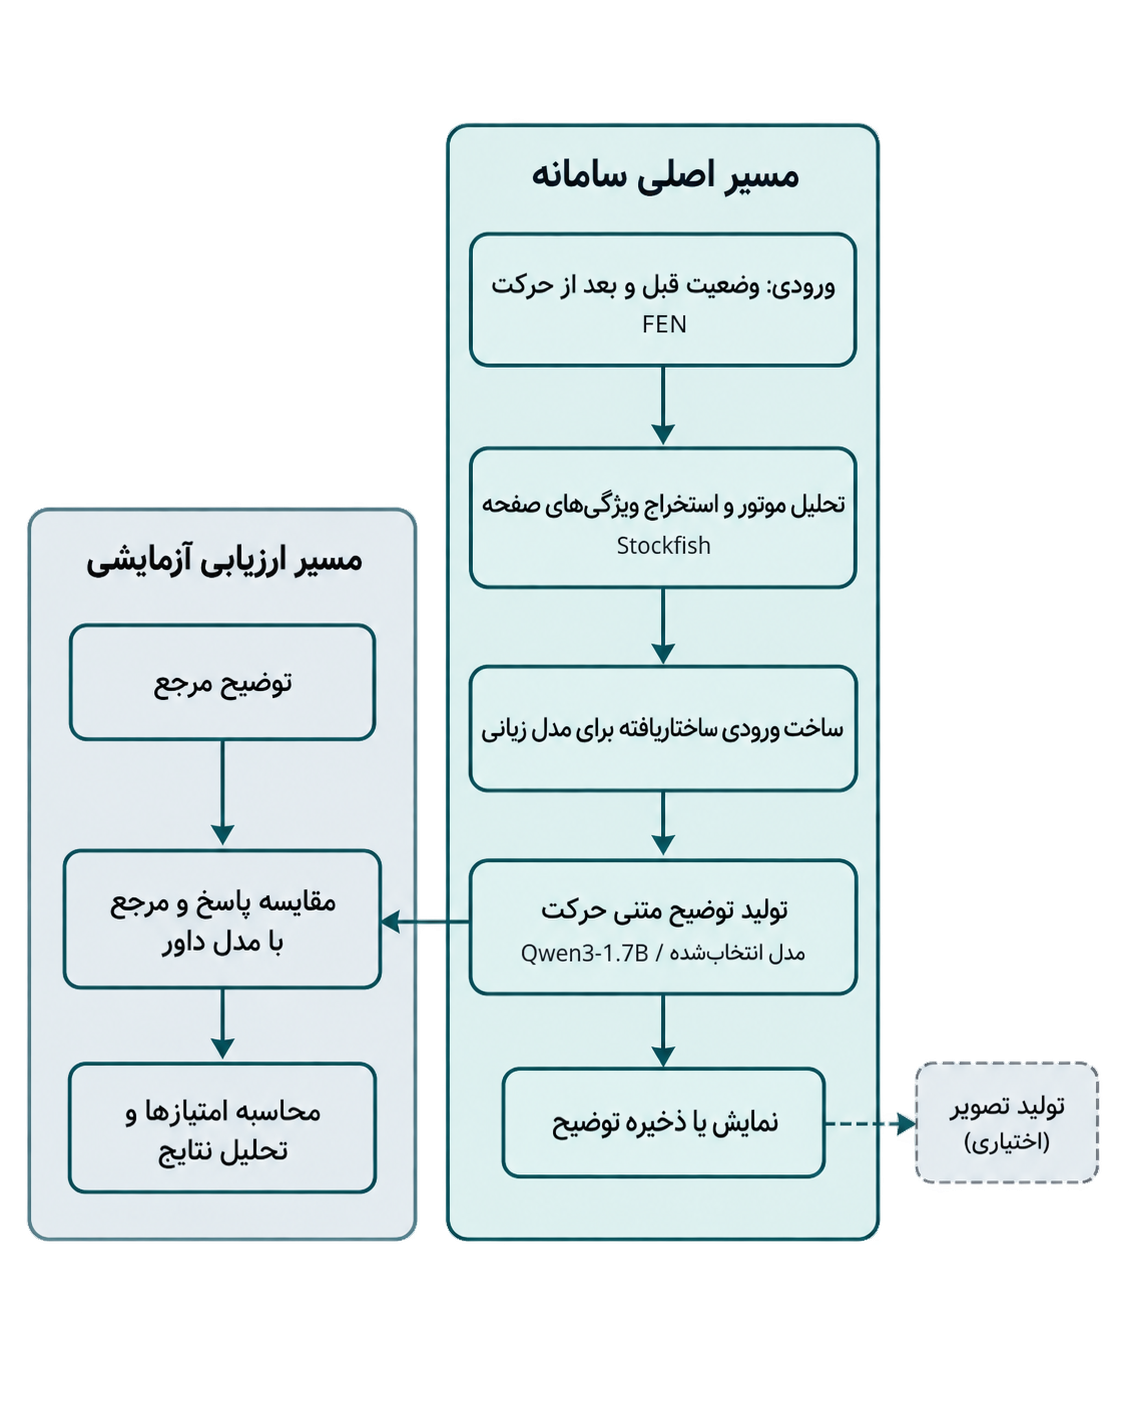
\includegraphics[width=0.93\linewidth]{chapter3_assets/pipeline_v2.png}
\caption{جریان پردازش و ارزیابی در سامانه پیشنهادی}
\label{fig:pipeline}
\end{figure}

\subsection{تحلیل موقعیت و استخراج ویژگی‌ها}
برای نمایش وضعیت صفحه از قالب \lr{FEN} استفاده می‌شود. این قالب علاوه بر محل مهره‌ها، اطلاعاتی مانند نوبت حرکت و حق قلعه‌رفتن را در اختیار بخش پردازش قرار می‌دهد. در پیاده‌سازی موجود، موتور با عمق جست‌وجوی ۱۷ فراخوانی می‌شود و تا سه ادامه پیشنهادی را بررسی می‌کند. تحلیل قبل و بعد از حرکت، شامل ارزیابی عددی و ادامه‌های پیشنهادی، بخشی از زمینه ورودی مدل زبانی را تشکیل می‌دهد. جهت ارزیابی باید ثابت بماند؛ در خروجی‌های ثبت‌شده، ارزیابی‌ها از دید سفید گزارش شده‌اند.

ماژول استخراج ویژگی‌ها برای هر دو رنگ اجرا می‌شود و تغییراتی مانند وجود مهره بدون دفاع، کاهش امنیت شاه، از دست رفتن کنترل مرکز، تأخیر در گسترش مهره‌ها و ضعف‌های ساختار پیاده‌ای را بررسی می‌کند. هدف این مرحله، برجسته‌کردن اطلاعاتی است که بیان آموزشی حرکت را آسان‌تر می‌سازند. این ویژگی‌ها حاصل قواعد پیاده‌سازی‌شده هستند و پوشش کامل تمام مفاهیم تاکتیکی و راهبردی شطرنج را تضمین نمی‌کنند. بنابراین، کنار هم قرار گرفتن ویژگی‌ها و تحلیل موتور به معنای تضمین صحت متن نهایی نیست؛ همین موضوع ضرورت ارزیابی مستقل خروجی را توضیح می‌دهد.

\subsection{ساخت ورودی و تولید توضیح}
در الگوی ورودی، از مدل خواسته می‌شود مانند یک مربی شطرنج، دلیل بهتر یا بدتر شدن موقعیت را در دو یا سه جمله کوتاه توضیح دهد. دستورها بر زبان ساده، بیان ایده به جای محاسبه و خودداری از تکرار نام حرکت‌ها، اعداد ارزیابی و خطوط موتور تأکید دارند. در نتیجه، میان «اطلاعاتی که مدل برای درک موقعیت دریافت می‌کند» و «اطلاعاتی که باید در متن آموزشی بازگو شود» تفاوت وجود دارد. مدل به شواهد عددی دسترسی دارد، اما باید پیامد آموزشی آن‌ها را بیان کند.

در کد پروژه دو روش تک‌مرحله‌ای و زنجیره‌ای پیش‌بینی شده است. روش تک‌مرحله‌ای مستقیماً از اطلاعات دو موقعیت و ویژگی‌های استخراج‌شده توضیح می‌سازد. در روش زنجیره‌ای، ابتدا برای موقعیت قبل و بعد توصیف جداگانه تولید می‌شود و سپس این توصیف‌ها در مرحله نهایی ترکیب می‌شوند. وجود این دو مسیر یک قابلیت نرم‌افزاری است؛ نتایج گزارش‌شده در این فصل، مقایسه کنترل‌شده این دو روش نیست و از آن‌ها نمی‌توان برتری یکی را نتیجه گرفت. مبنای مقایسه عددی، پاسخ‌های ذخیره‌شده مدل‌ها برای مجموعه مشترک آزمون است.

\subsection{مدل محلی و رابط کاربری}
در کنار مدل‌های عمومی، مدل کوچک اختصاصی با شناسه \lr{chess-q8\_0} ارزیابی شده است. مطابق دفترچه آموزش پروژه، مدل پایه \lr{Qwen3-1.7B} با \lr{۱٫۷} میلیارد پارامتر است و با روش \lr{LoRA} بر متن کتاب‌های شطرنج سازگار شده است. نسخه آزموده‌شده با کمی‌سازی \lr{Q8\_0} از طریق \lr{llama.cpp} به صورت محلی اجرا می‌شود. آموزش روی متن کتاب با آموزش نظارت‌شده بر جفت‌های «موقعیت و توضیح صحیح همان موقعیت» یکسان نیست؛ ازاین‌رو، آشنایی با ادبیات شطرنج لزوماً به اتصال درست متن به وضعیت صفحه منجر نمی‌شود. اندازه کوچک این مدل، مقایسه کیفیت آن با نسخه‌های بزرگ‌تر را به یکی از جنبه‌های مهم این آزمایش تبدیل می‌کند.

شکل~\ref{fig:ui} تصویر موجود در مستندات پروژه از رابط کاربری را نشان می‌دهد. صفحه شطرنج و بخش توضیح در کنار هم قرار گرفته‌اند تا کاربر بتواند متن را همراه وضعیت بازی مشاهده کند. این تصویر برای معرفی شکل ارائه خروجی استفاده شده است و نمونه‌ای از اثبات صحت تحلیل یا بخشی از نتایج کمی آزمون محسوب نمی‌شود.

\begin{figure}[htbp]
\centering
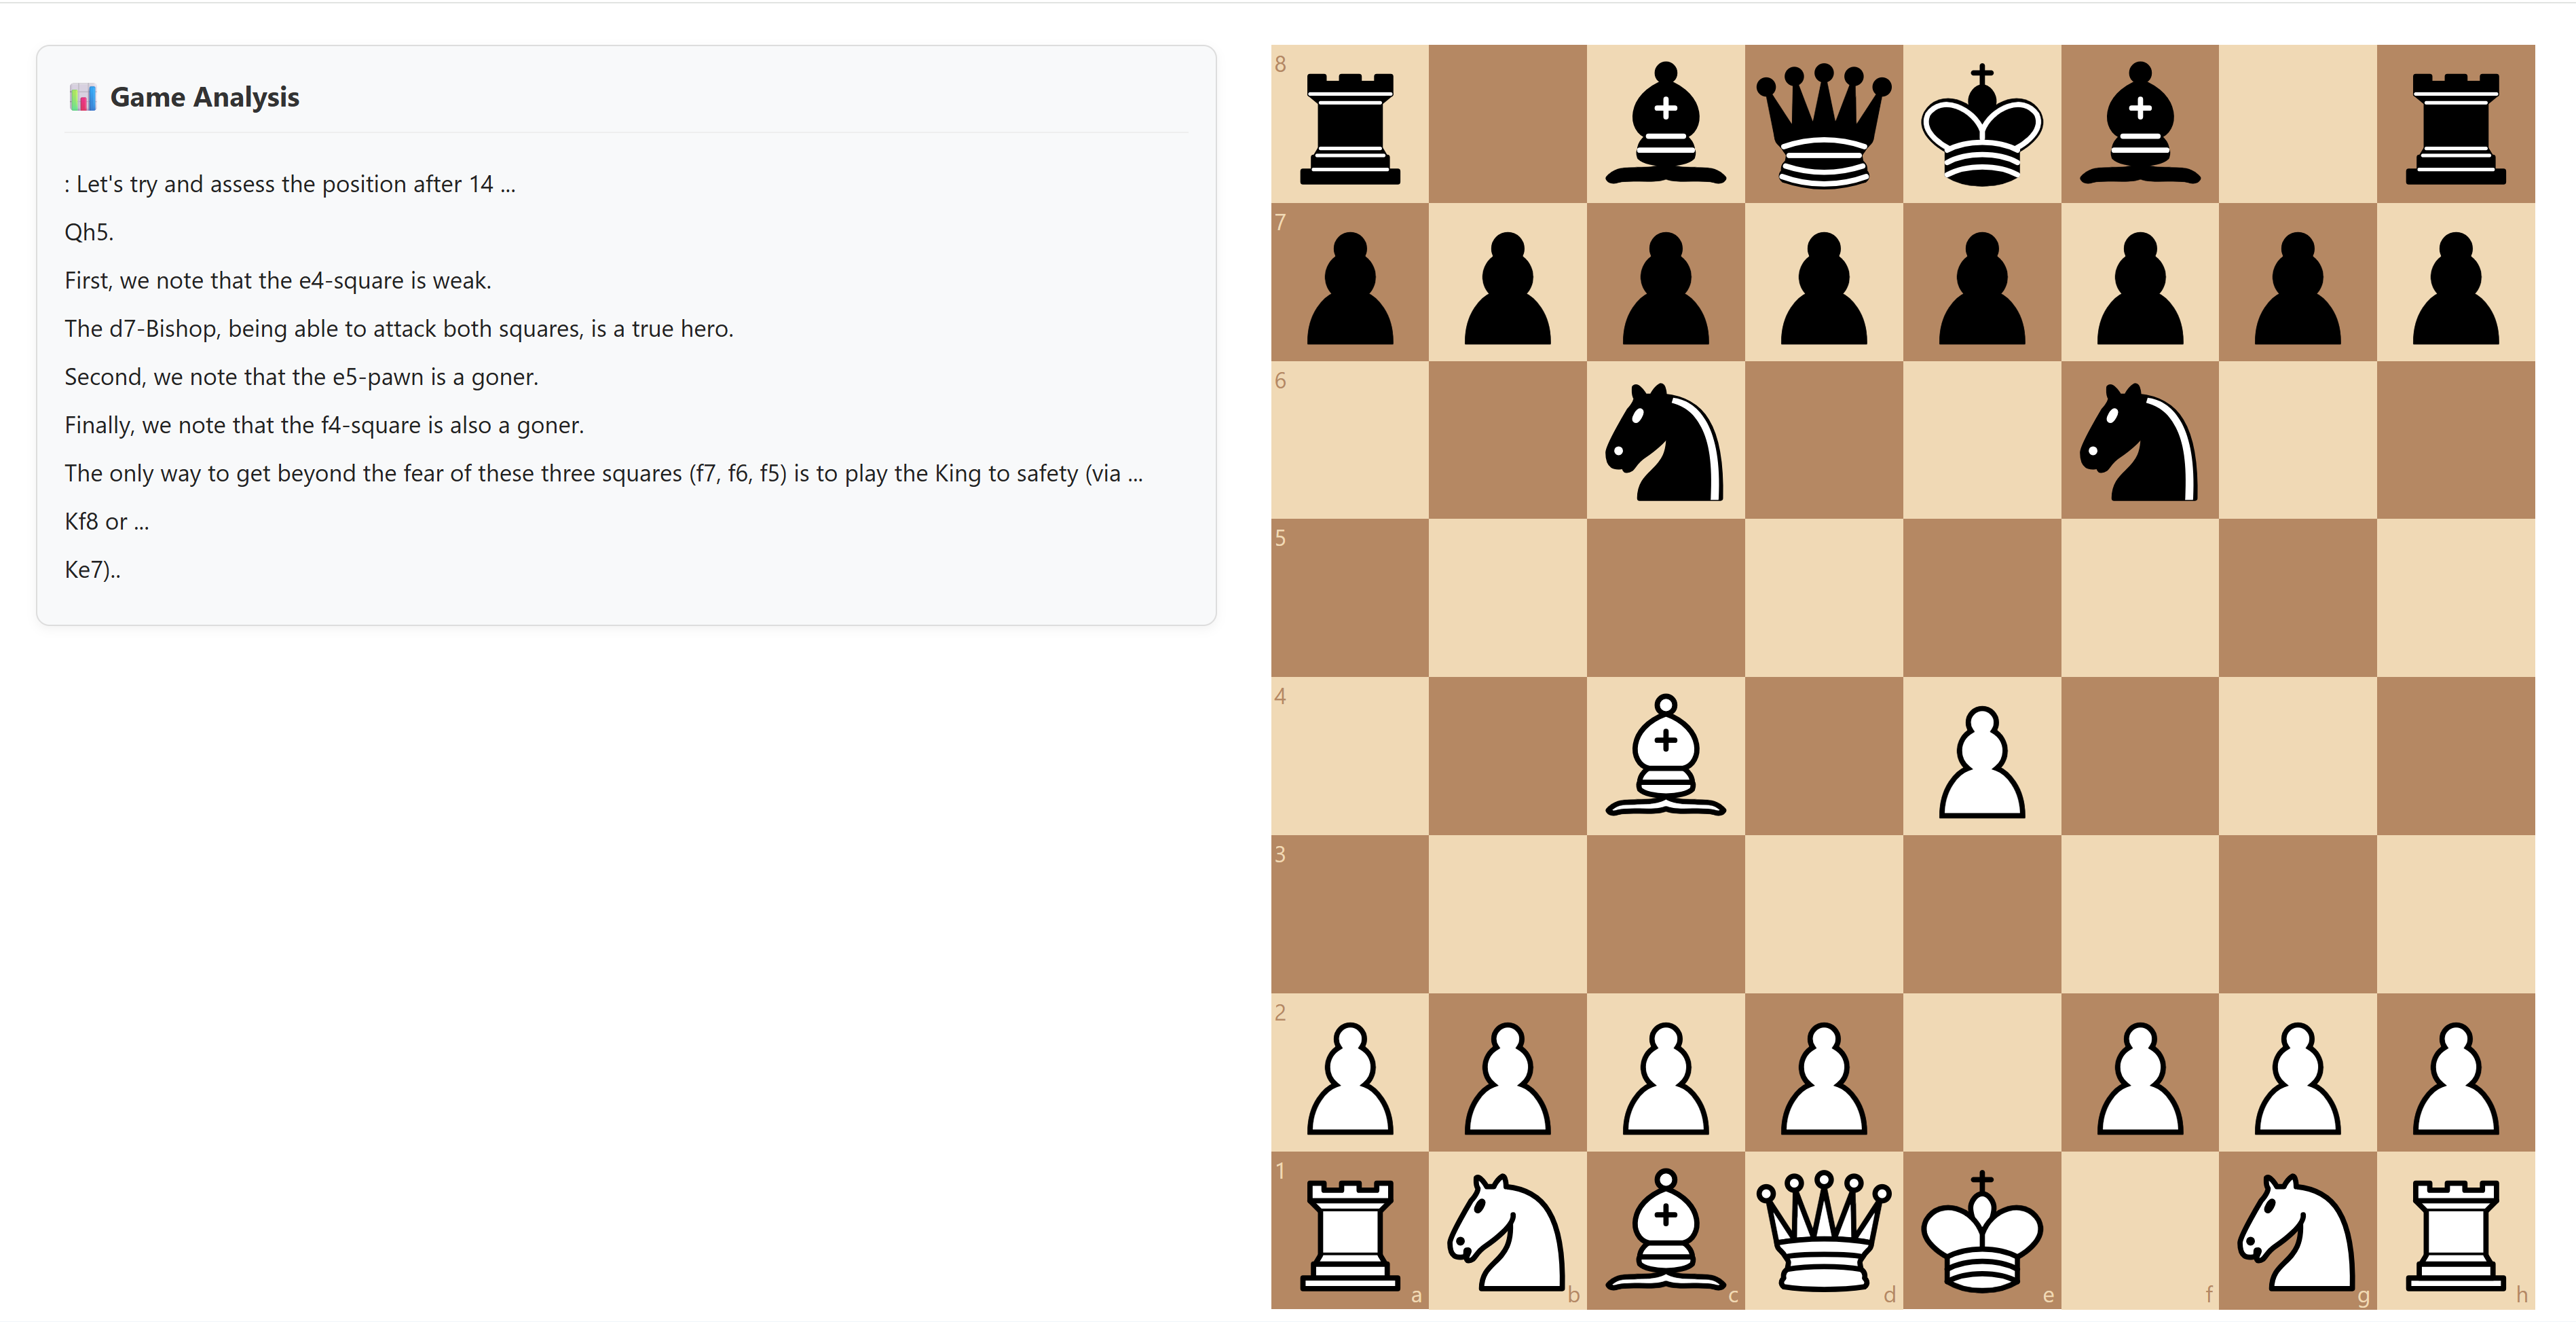
\includegraphics[width=\linewidth]{software_screenshot.png}
\caption{تصویر رابط کاربری ثبت‌شده در مستندات پروژه}
\label{fig:ui}
\end{figure}

\section{روش ارزیابی آزمایشی}
\subsection{تهیه و ساختار مجموعه آزمون}
مجموعه نهایی ارزیابی در پرونده \lr{evaluation\_dataset.tsv} شامل ۶۰ نمونه است. هر نمونه یک انتقال از وضعیت قبل به وضعیت بعد از حرکت را توصیف می‌کند. مجموعه به صورت متوازن از سه گروه مبتدی، متوسط و پیشرفته تشکیل شده و در هر گروه ۲۰ نمونه وجود دارد. همان‌طور که در فصل اول بیان شد، نمونه‌ها و توضیحات مرجع به صورت دستی بررسی و برچسب‌گذاری شده‌اند.

در اسکریپت دسته‌بندی بازی‌ها، میانگین امتیاز دو بازیکن مبنای گروه‌بندی است: کمتر از ۱۲۰۰ برای مبتدی، از ۱۲۰۰ تا کمتر از ۱۸۰۰ برای متوسط و ۱۸۰۰ و بالاتر برای پیشرفته. بازی‌های کوتاه‌تر از ۳۰ نیم‌حرکت کنار گذاشته می‌شوند. باید توجه داشت که سطح بازیکنان فقط مبنای دسته‌بندی منبع نمونه‌هاست و اندازه‌گیری مستقلی از دشواری تاکتیکی تک‌تک موقعیت‌ها نیست. همچنین تعداد بازی‌های اولیه با تعداد نمونه‌های نهایی آزمون تفاوت دارد؛ واحد محاسبه امتیاز در این فصل، یک موقعیت‌ـ‌حرکت است.

\begin{table}[htbp]
\centering
\caption{ترکیب مجموعه آزمون نهایی}
\label{tab:dataset}
\begin{tabular}{lrrr}
\toprule
گروه & تعداد نمونه & سهم از مجموعه & میانگین امتیاز بازیکنان در دسته‌بندی \\
\midrule
مبتدی & ۲۰ & \lr{۳۳٫۳} درصد & کمتر از ۱۲۰۰ \\
متوسط & ۲۰ & \lr{۳۳٫۳} درصد & ۱۲۰۰ تا کمتر از ۱۸۰۰ \\
پیشرفته & ۲۰ & \lr{۳۳٫۳} درصد & ۱۸۰۰ و بیشتر \\
\midrule
مجموع & ۶۰ & ۱۰۰ درصد & \lr{---} \\
\bottomrule
\end{tabular}
\end{table}

برای هر نمونه، شناسه، وضعیت قبل و بعد، حرکت، ورودی مدل، توضیح مرجع و گروه سطح ذخیره شده است. پاسخ‌های تولیدی نیز در پرونده‌های جداگانه با نام مدل نگهداری می‌شوند. در مرحله داوری، کلید ترکیبی «گروه و شناسه نمونه» برای تطبیق پاسخ و مرجع به کار می‌رود. این انتخاب اهمیت دارد، زیرا شناسه محلی یک حرکت ممکن است در گروه دیگری تکرار شود و تطبیق صرفاً بر اساس ترتیب سطرها یا شناسه تنها، قابل اتکا نیست.

\subsection{مدل‌های مقایسه‌شده و محدوده آزمایش}
در این ارزیابی، ۱۱ مدل پاسخ‌دهنده بررسی شده‌اند. شناسه‌های ثبت‌شده شامل مدل اختصاصی \lr{chess-q8\_0} و مدل‌های \lr{Llama-3.2-3B-Instruct-Q4\_K\_M}، \lr{gemma-3-12b-it-Q4\_0}، \lr{qwen3-30b-a3b}، \lr{gpt-oss-120b}، \lr{cf.llama-3.3-70b-instruct-fp8-fast}، \lr{cf.gemma-4-26b-a4b-it}، \lr{grok-4.3}، \lr{gemini-3.5-flash}، \lr{qwen3.7-plus} و \lr{gpt-5.5} هستند. نام‌های کوتاه‌تر در نمودارها و جدول نتایج به همین شناسه‌ها اشاره دارند و ادعایی درباره مشخصات منتشرنشده مدل‌ها ندارند.

هر مدل ۶۰ پاسخ در فایل ارزیابی دارد؛ بنابراین تحلیل اصلی بر ۶۶۰ رکورد داوری استوار است. مدل داور در تمام این پرونده‌ها با شناسه \lr{gemma4-12b} ثبت شده است. خروجی داورهای دیگر که در پوشه‌های جداگانه پروژه وجود دارند، در این مقایسه وارد نشده‌اند تا مبنای امتیازدهی ثابت بماند. یکسان بودن مجموعه آزمون، به معنای یکسان بودن سخت‌افزار، هزینه، تأخیر یا تنظیمات داخلی سرویس‌های مختلف نیست؛ داده‌های این آزمایش برای مقایسه کیفیت پاسخ استفاده می‌شوند.

\subsection{معیارهای داوری و محاسبه امتیاز}
داور، متن پاسخ و توضیح مرجع را دریافت می‌کند و برای پنج معیار مستقل، عددی بین صفر و ده برمی‌گرداند. در دستور داوری، مرجع مبنای قضاوت است؛ بازنویسی هم‌معنا پذیرفته می‌شود و ادعاهای قوی بدون پشتوانه، مانند مات اجباری یا کسب قطعی مهره، باید امتیاز صحت و وفاداری را کاهش دهند. داور در این مرحله صفحه را با موتور تحلیل نمی‌کند. بنابراین، «صحت» در این آزمایش به توافق با واقعیت‌های بیان‌شده در مرجع اشاره دارد و معادل اثبات مستقل تمام ادعاهای شطرنجی نیست.

\begin{table}[htbp]
\centering
\caption{معیارها و وزن آن‌ها در امتیاز نهایی}
\label{tab:criteria}
\begin{tabular}{rp{9cm}r}
\toprule
معیار & تعریف عملیاتی & وزن \\
\midrule
صحت & انطباق ادعاهای اصلی پاسخ با واقعیت‌های توضیح مرجع & ۳۵ درصد \\
وفاداری & پایبندی به مرجع و پرهیز از افزودن ادعای بدون پشتوانه & ۲۵ درصد \\
مفیدبودن & انتقال روشن درس، علت یا پیامد آموزشی حرکت & ۲۰ درصد \\
پیروی از دستور & ارائه توضیح مرتبط و مناسب مخاطب یادگیرنده & ۱۰ درصد \\
روانی & درستی زبانی، خوانایی و وضوح متن & ۱۰ درصد \\
\bottomrule
\end{tabular}
\end{table}

امتیاز کلی در برنامه محاسبه می‌شود و از داور درخواست نمی‌شود آن را مستقیماً تولید کند. اگر صحت، وفاداری، مفیدبودن، پیروی از دستور و روانی به‌ترتیب با $C$، $F$، $H$، $I$ و $L$ نمایش داده شوند، امتیاز هر پاسخ برابر است با:
\begin{equation}
S=0.35C+0.25F+0.20H+0.10I+0.10L.
\end{equation}
در نتیجه، صحت و وفاداری روی هم ۶۰ درصد وزن نهایی را تشکیل می‌دهند. میانگین امتیاز ۶۰ پاسخ، نتیجه هر مدل را تعیین می‌کند و برای مقایسه گروه‌ها، میانگین ۲۰ پاسخ همان گروه محاسبه می‌شود. میانگین امتیازها در جدول‌ها با دو رقم اعشار نمایش داده شده است.

پیروی از دستور در متن داوری بیشتر بر مرتبط و آموزشی بودن پاسخ تأکید دارد؛ ازاین‌رو، امتیاز بالای این معیار الزاماً به معنای رعایت دقیق تعداد جمله‌ها یا پرهیز کامل از نمادگذاری حرکت نیست. این تفاوت باید در تفسیر نتایج در نظر گرفته شود. پاسخ داور نیز از نظر ساختار و دامنه اعداد بررسی می‌شود. در ۶۶۰ رکورد این مقایسه خطای تجزیه خروجی داور ثبت نشده است؛ بااین‌حال، نبود خطای ساختاری به معنای نبود خطای قضاوت نیست.

\subsection{ابزارها، منابع داده و دسترسی‌ها}
منابع داخلی این فصل شامل مجموعه آزمون، پرونده‌های پاسخ و داوری، کد تحلیل شطرنج و تصویر رابط کاربری است. مسیر داده بازی‌ها در اسکریپت دسته‌بندی به آرشیو بازی‌های استاندارد امتیازدار \lr{Lichess}~\cite{lichess-data} در فوریه ۲۰۱۳ اشاره دارد. مطالعه کاربری با شرکت‌کنندگان انسانی در نتایج حاضر گزارش نشده و ارزیابی کمی بر داده‌های ذخیره‌شده و داوری خودکار تکیه دارد. همچنین اندازه‌گیری مستقلی از زمان پاسخ، مصرف حافظه یا انرژی در این مجموعه نتایج وجود ندارد؛ بنابراین برای این شاخص‌ها عددی ارائه نمی‌شود.

در پرونده‌های بررسی‌شده، سند مجوز ویژه یا تأییدیه اخلاق برای این آزمایش ثبت نشده است. این بیان به معنی آزاد بودن بازنشر همه منابع نیست؛ برای انتشار مستقل متن کتاب‌های آموزشی یا داده‌های منبع باید وضعیت مجوز همان منابع بررسی شود. در این فصل از بازنشر متن کتاب‌ها استفاده نشده و تصاویر، خروجی‌های موجود خود پروژه هستند.

\section{نتایج و تحلیل}
\subsection{مقایسه کلی مدل‌ها}
جدول~\ref{tab:results} میانگین سه معیار محتوایی و امتیاز وزنی نهایی مدل‌ها را نشان می‌دهد. مدل \lr{GPT-5.5} با امتیاز \lr{۷٫۳۱} در این مجموعه رتبه نخست را دارد. پس از آن، \lr{Qwen3.7 Plus} با \lr{۶٫۵۰} و \lr{Gemini 3.5 Flash} با \lr{۶٫۴۶} قرار می‌گیرند. اختلاف دو مدل اخیر حدود \lr{۰٫۰۴} امتیاز است؛ بدون آزمون آماری و بررسی عدم‌قطعیت، نباید این فاصله کوچک را نشانه برتری قطعی دانست.

\begin{table}[htbp]
\centering\small
\caption{میانگین نتایج ۱۱ مدل؛ ۶۰ نمونه برای هر مدل و مقیاس صفر تا ده}
\label{tab:results}
\begin{tabular}{lrrrr}
\toprule
مدل پاسخ‌دهنده & صحت & وفاداری & مفیدبودن & امتیاز کلی \\
\midrule
\lr{GPT-5.5} & \lr{6.28} & \lr{6.43} & \lr{7.57} & \lr{7.31} \\
\lr{Qwen3.7 Plus} & \lr{5.30} & \lr{5.27} & \lr{6.63} & \lr{6.50} \\
\lr{Gemini 3.5 Flash} & \lr{5.15} & \lr{5.27} & \lr{6.70} & \lr{6.46} \\
\lr{Grok 4.3} & \lr{3.92} & \lr{4.08} & \lr{5.27} & \lr{5.44} \\
\lr{Llama 3.3 70B (FP8)} & \lr{2.20} & \lr{2.53} & \lr{3.65} & \lr{4.12} \\
\lr{GPT-OSS 120B} & \lr{2.10} & \lr{2.17} & \lr{3.47} & \lr{3.97} \\
\lr{Qwen3 30B A3B} & \lr{1.65} & \lr{1.85} & \lr{2.87} & \lr{3.59} \\
\lr{Gemma 3 12B (Q4)} & \lr{0.88} & \lr{0.92} & \lr{2.03} & \lr{2.95} \\
\lr{Gemma 4 26B A4B} & \lr{0.82} & \lr{0.88} & \lr{2.00} & \lr{2.90} \\
\lr{Chess Q8 (Qwen3 1.7B)} & \lr{0.98} & \lr{1.08} & \lr{2.17} & \lr{2.86} \\
\lr{Llama 3.2 3B (Q4)} & \lr{0.83} & \lr{0.93} & \lr{1.95} & \lr{2.86} \\

\bottomrule
\end{tabular}
\end{table}

مدل اختصاصی مبتنی بر \lr{Qwen3-1.7B} میانگین \lr{۲٫۸۵۸۳} را کسب کرده است که با دو رقم اعشار \lr{۲٫۸۶} گزارش می‌شود. میانگین \lr{Llama 3.2 3B} برابر با \lr{۲٫۸۵۵۰} است؛ بنابراین هر دو در نمایش دورقمی امتیاز \lr{۲٫۸۶} دارند و اختلاف بسیار کوچک آن‌ها نباید به عنوان برتری معنادار تفسیر شود. امتیاز مدل کوچک همچنین به \lr{Gemma 4 26B A4B} با \lr{۲٫۹۰} و \lr{Gemma 3 12B} با \lr{۲٫۹۵} نزدیک است؛ فاصله با این دو مدل به‌ترتیب حدود \lr{۰٫۰۴} و \lr{۰٫۰۹} امتیاز است. در مقابل، فاصله آن با بهترین مدل این آزمایش حدود \lr{۴٫۴۵} امتیاز باقی می‌ماند.

\begin{figure}[htbp]
\centering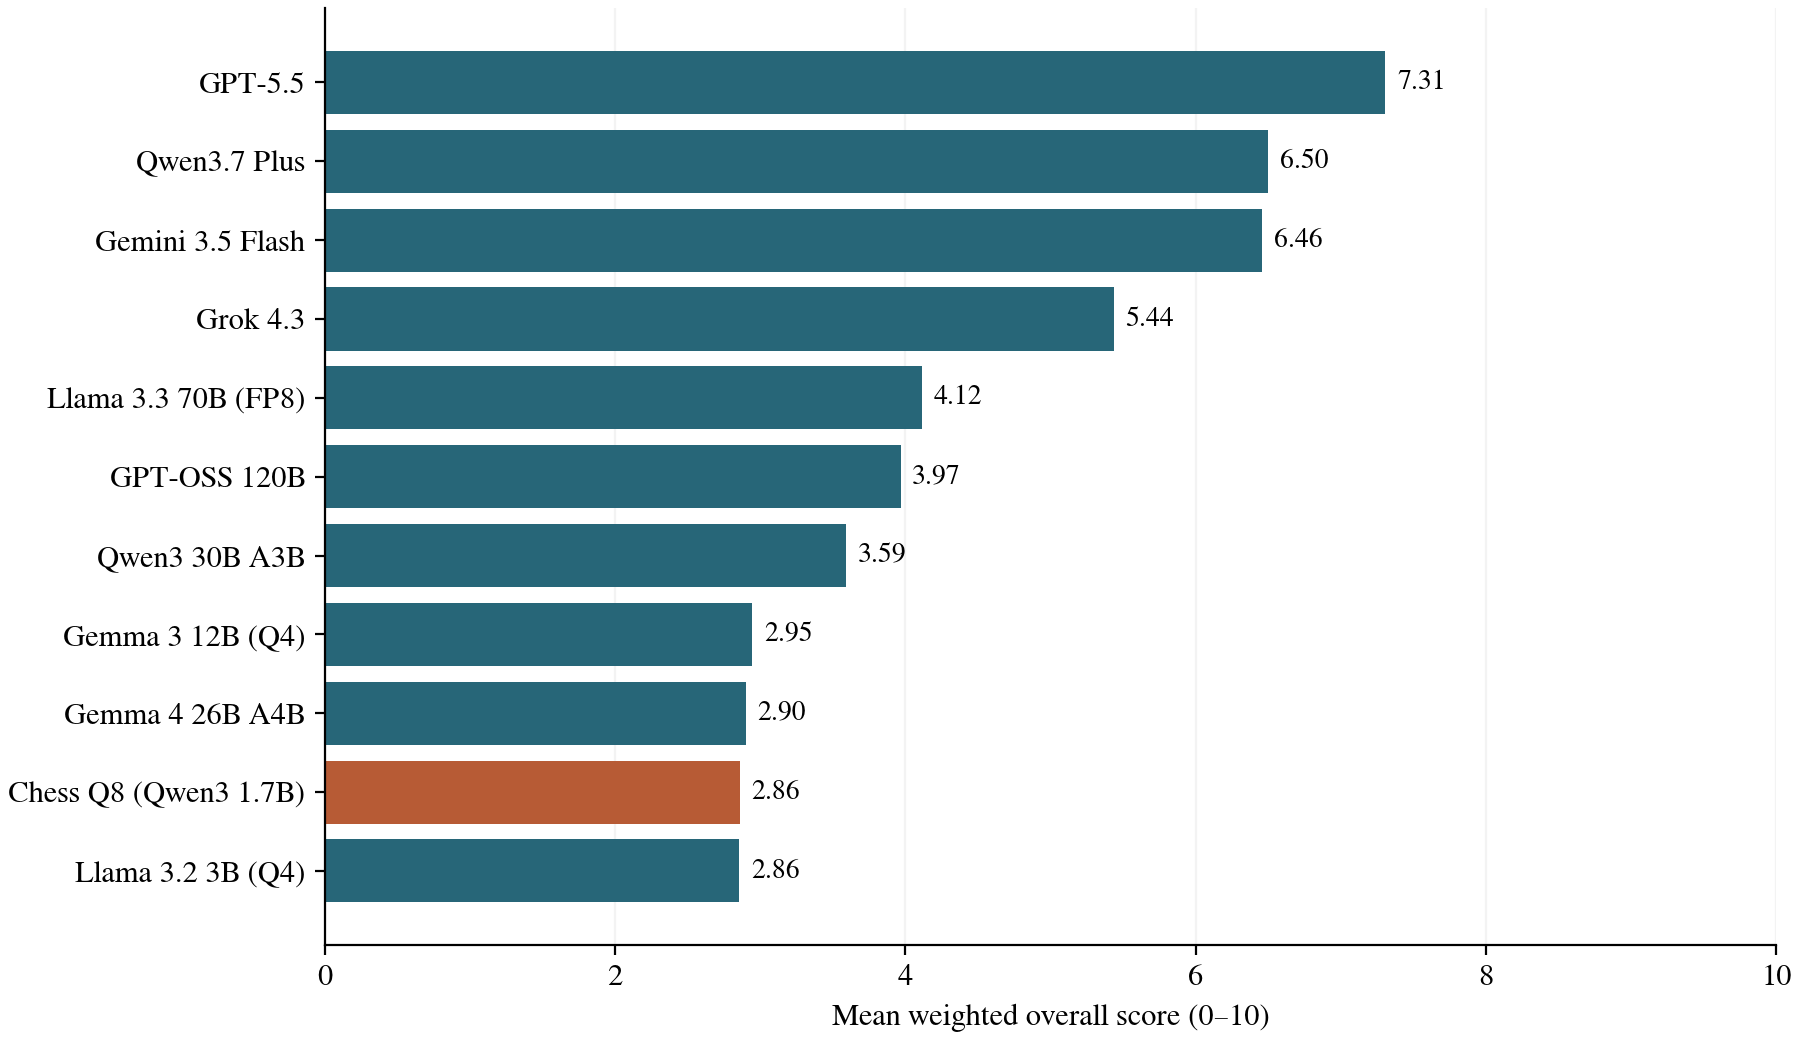
\includegraphics[width=\linewidth]{chapter3_assets/overall.png}
\caption{رتبه‌بندی میانگین امتیاز وزنی؛ داور ثابت و ۶۰ نمونه برای هر مدل}
\label{fig:overall}
\end{figure}


\subsection{جایگاه مدل کوچک در مقایسه با مدل‌های بزرگ‌تر}
شکل~\ref{fig:smallmodel} امتیاز مدل اختصاصی مبتنی بر \lr{Qwen3-1.7B} را در کنار چند مدل بزرگ‌تر نشان می‌دهد. مدل \lr{۱٫۷} میلیاردپارامتری با امتیاز \lr{۲٫۸۶} به میانگین مدل ۳ میلیاردپارامتری \lr{Llama 3.2} و دو مدل \lr{Gemma} نزدیک است. این مقایسه، مکمل رتبه‌بندی کامل ۱۱ مدل در شکل~\ref{fig:overall} است و فقط بخشی از مدل‌های آزموده‌شده را برجسته می‌کند.

\begin{figure}[htbp]
\centering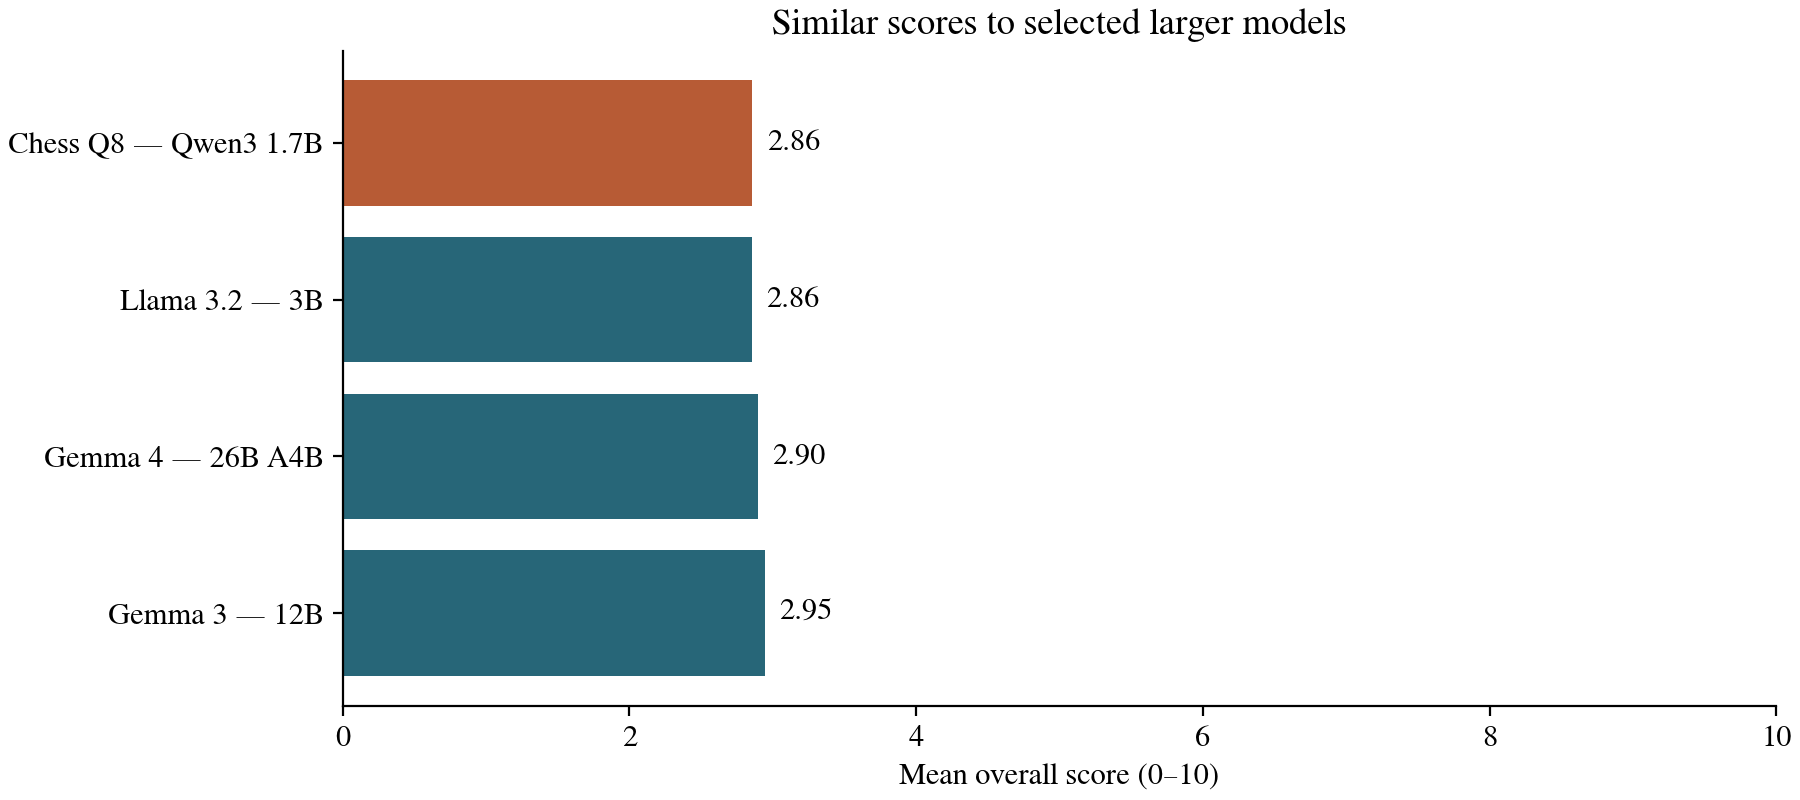
\includegraphics[width=\linewidth]{chapter3_assets/small_model_comparison.png}
\caption{مقایسه امتیاز مدل اختصاصی \lr{۱٫۷} میلیاردپارامتری با چند مدل بزرگ‌تر بر روی ۶۰ نمونه مشترک}
\label{fig:smallmodel}
\end{figure}

نزدیکی امتیاز مدل \lr{۱٫۷} میلیاردپارامتری به چند مدل با اندازه اسمی بیشتر، نتیجه‌ای امیدوارکننده برای بررسی کاربرد مدل‌های کوچک در این مسئله است. این نتیجه نشان می‌دهد که در مجموعه حاضر، اندازه بیشتر به تنهایی تضمین‌کننده امتیاز بهتر نیست. بااین‌حال، مدل‌ها از نظر آموزش، معماری، کمی‌سازی و تنظیمات اجرا یکسان نیستند؛ به‌ویژه شناسه \lr{26B A4B} به مدلی با معماری متخصص‌های ترکیبی اشاره دارد و تعداد کل پارامترها با تعداد پارامترهای فعال برابر نیست. از این مقایسه نمی‌توان نسبت مستقیم سرعت، مصرف حافظه یا هزینه را استخراج کرد. همچنین آزمون برابری آماری انجام نشده است؛ تعبیر دقیق نتیجه، «نزدیکی میانگین امتیازها در این آزمایش» است، نه برابری عمومی قابلیت مدل‌ها.

\subsection{تفاوت روانی متن و صحت محتوایی}
شکل~\ref{fig:metrics} پنج معیار را به صورت جداگانه نمایش می‌دهد. در ده مدل، میانگین روانی برابر با ۱۰ است؛ برای مدل اختصاصی نیز روانی حدود \lr{۹٫۹۷} به دست آمده است. بااین‌حال، صحت حدود \lr{۰٫۹۸}، وفاداری حدود \lr{۱٫۰۸}، مفیدبودن حدود \lr{۲٫۱۷} و پیروی از دستور حدود \lr{۸٫۱۳} هستند. پس نزدیکی امتیاز کلی به چند مدل بزرگ‌تر، نباید ضعف باقی‌مانده در معیارهای محتوایی را پنهان کند. متن می‌تواند از نظر جمله‌بندی مناسب باشد و همچنان پیام اصلی مرجع را منتقل نکند یا ادعایی ناسازگار با آن بسازد.

\begin{figure}[htbp]
\centering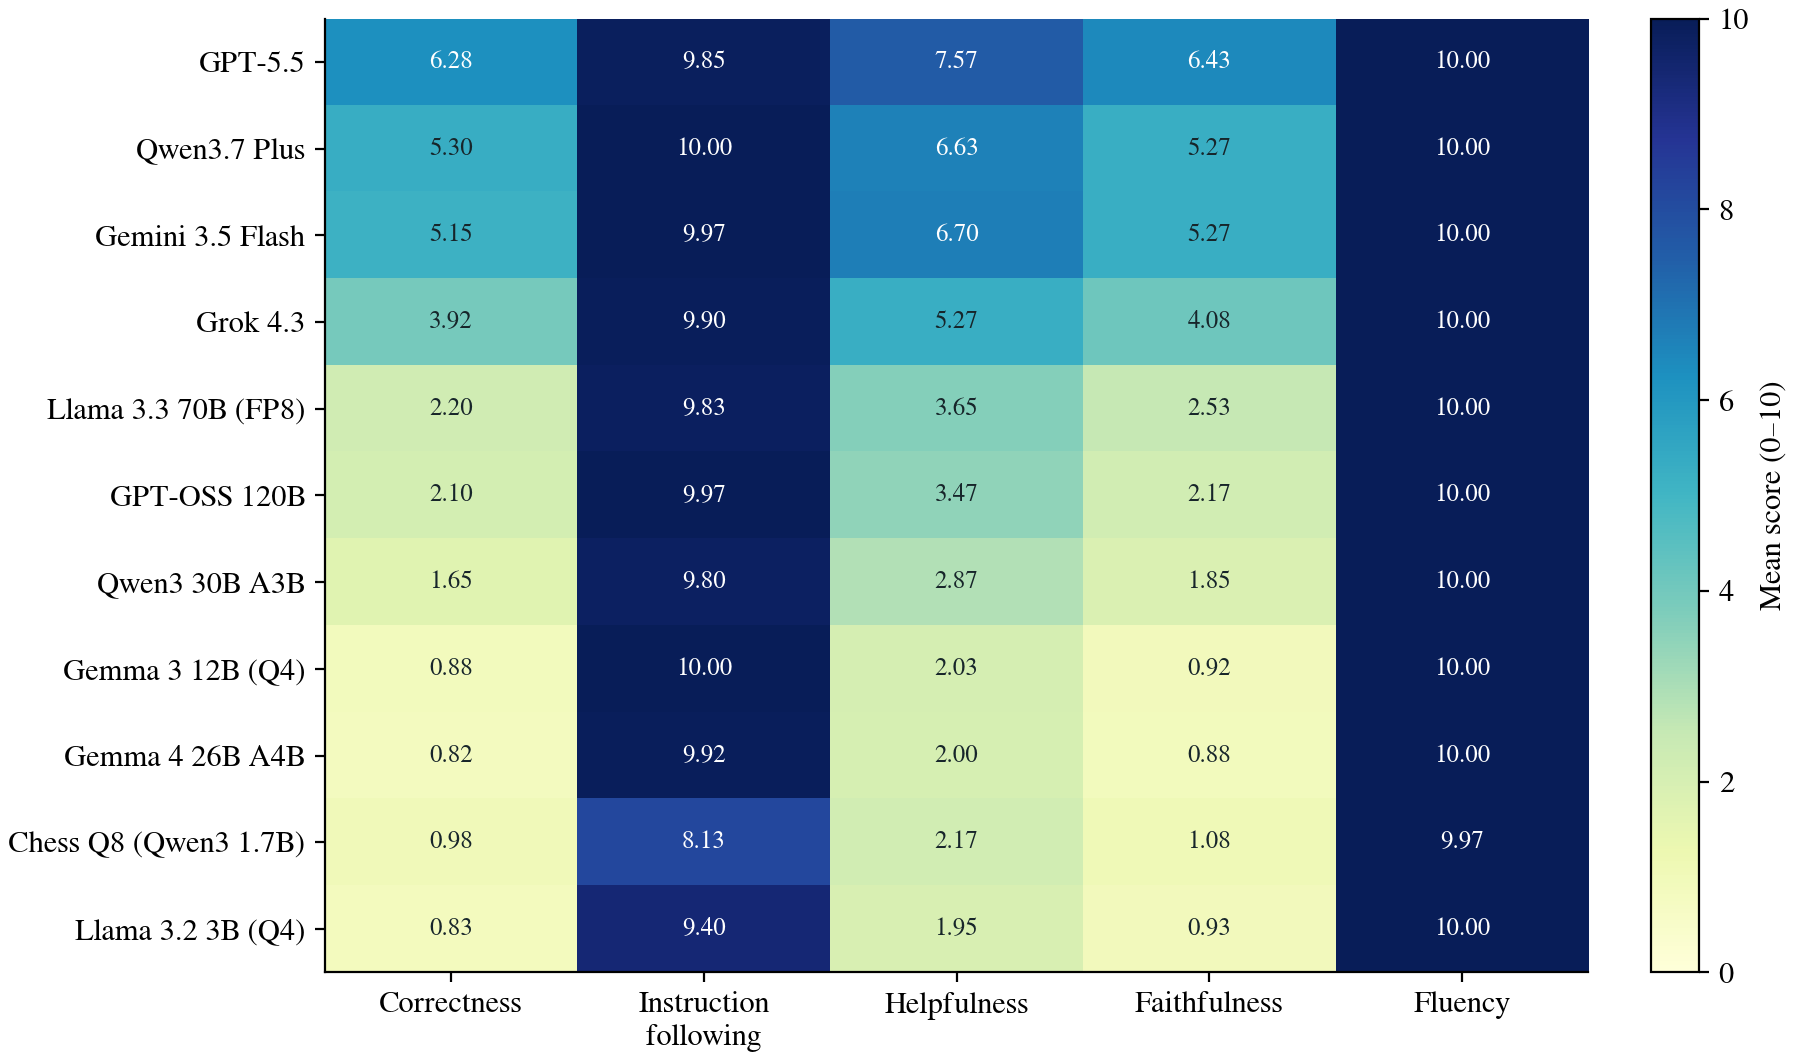
\includegraphics[width=\linewidth]{chapter3_assets/metrics.png}
\caption{میانگین پنج معیار داوری؛ رنگ تیره‌تر نشان‌دهنده امتیاز بیشتر است}
\label{fig:metrics}
\end{figure}

نزدیک بودن امتیازهای روانی به سقف مقیاس، توان تمایز این معیار را در آزمایش حاضر کاهش می‌دهد. از سوی دیگر، چون معیارهای صحت و وفاداری هر دو به مرجع وابسته‌اند، نباید آن‌ها را دو تأیید کاملاً مستقل از درستی شطرنجی فرض کرد. با این ملاحظه، نتیجه اصلی همچنان روشن است: برای انتخاب مدل آموزشی، تکیه بر خوانایی متن یا ظاهر تخصصی پاسخ کافی نیست و معیارهای محتوایی باید نقش اصلی داشته باشند.

\subsection{نتایج به تفکیک سطح نمونه‌ها}
شکل~\ref{fig:categories} امتیاز کلی را برای هر گروه نمایش می‌دهد. امتیاز \lr{GPT-5.5} در گروه‌های مبتدی، متوسط و پیشرفته به‌ترتیب \lr{۷٫۳۶}، \lr{۷٫۸۵} و \lr{۶٫۷۲} است. برای \lr{Gemini 3.5 Flash} این مقادیر \lr{۷٫۱۰}، \lr{۷٫۰۸} و \lr{۵٫۱۹} هستند. کاهش امتیاز در گروه پیشرفته برای این مدل‌ها با دشوارتر بودن انتقال مضمون برخی موقعیت‌ها سازگار است، اما به‌تنهایی رابطه علّی میان سطح بازیکن و کیفیت توضیح را اثبات نمی‌کند.

\begin{figure}[htbp]
\centering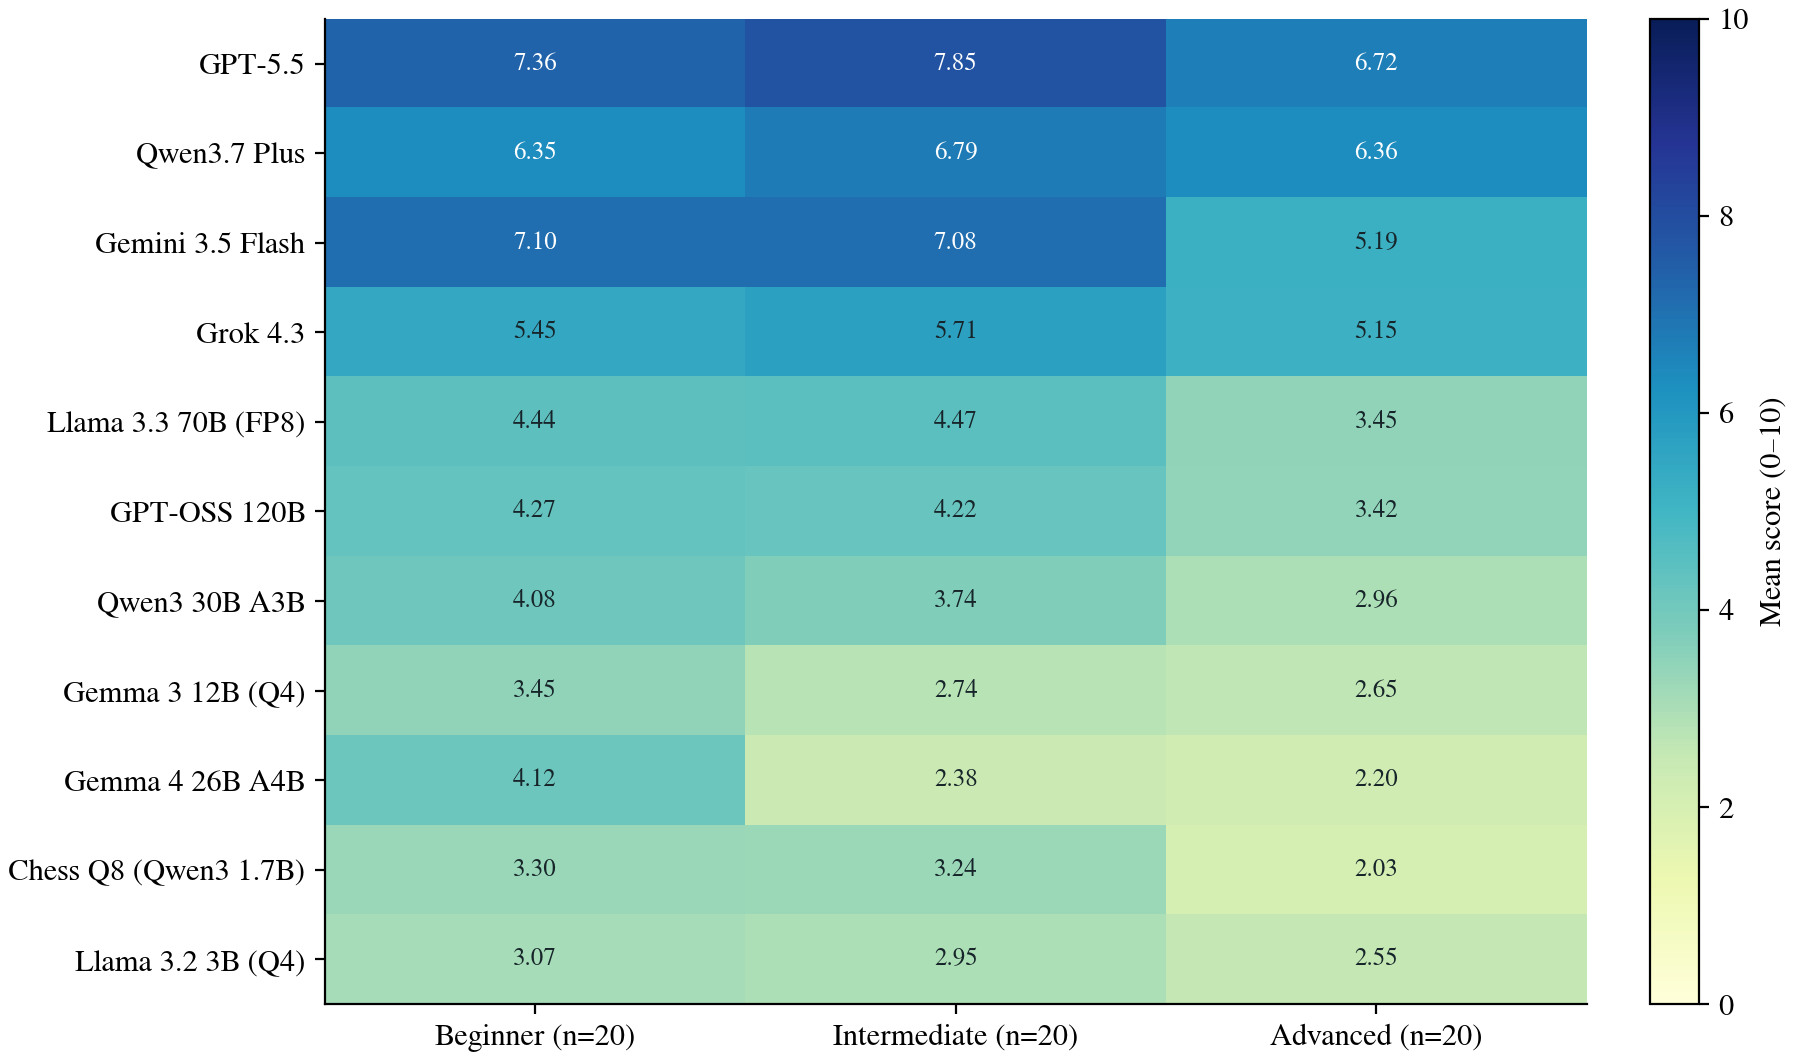
\includegraphics[width=\linewidth]{chapter3_assets/categories.png}
\caption{میانگین امتیاز کلی به تفکیک گروه؛ هر خانه حاصل ۲۰ نمونه است}
\label{fig:categories}
\end{figure}

مدل \lr{Qwen3.7 Plus} در سه گروه به‌ترتیب \lr{۶٫۳۵}، \lr{۶٫۷۹} و \lr{۶٫۳۶} امتیاز دارد و نسبت به دو مدل یادشده تغییر کمتری نشان می‌دهد. مدل اختصاصی نیز در گروه مبتدی \lr{۳٫۳۰}، متوسط \lr{۳٫۲۴} و پیشرفته \lr{۲٫۰۳} امتیاز گرفته است. این الگو نشان می‌دهد بررسی میانگین کلی به تنهایی کافی نیست؛ مدل مناسب باید علاوه بر کیفیت متوسط، در نوع موقعیت مورد استفاده نیز بررسی شود. با وجود توازن تعداد نمونه‌ها، هر گروه فقط ۲۰ نمونه دارد و تعمیم نتیجه به تمام بازی‌های آن سطح نیازمند مجموعه بزرگ‌تر است.

\subsection{بررسی یک نمونه واقعی}
شکل~\ref{fig:example} نمونه \lr{g1\_m38} از گروه پیشرفته را نشان می‌دهد. حرکت ثبت‌شده \lr{Bxf8} است و تصویر، موقعیت قبل و بعد از گرفتن رخ با فیل سفید را نمایش می‌دهد. توضیح مرجع بر این نکته تأکید دارد که ارزش ظاهری گرفتن رخ نباید پیامد تاکتیکی ادامه بازی را پنهان کند: پاسخ حریف تهدیدی علیه وزیر ایجاد می‌کند و دنباله تعویض‌ها می‌تواند به زیان سفید تمام شود. این توصیف، خلاصه پیام مرجع ذخیره‌شده است، نه تحلیل تازه‌ای که جداگانه توسط موتور تأیید شده باشد.

\begin{figure}[htbp]
\centering
\includegraphics[width=\linewidth]{../../artifacts/analysis_images/g1_m38__model_chess-q8_0.png}
\caption{نمونه واقعی گروه پیشرفته؛ وضعیت قبل در چپ و وضعیت بعد در راست}
\label{fig:example}
\end{figure}

پاسخ مدل اختصاصی در همین نمونه، به حرکت‌های دیگری مانند \lr{Nxe4} و \lr{Nxc3} اشاره کرده و پیامد حرکت را با حمله به شاه و کنترل صفحه توضیح داده است. این پاسخ با درس اصلی مرجع هم‌راستا نیست. داور برای صحت، وفاداری و مفیدبودن آن امتیاز صفر و برای روانی و پیروی از دستور امتیاز ده ثبت کرده است؛ حاصل وزنی برابر با \lr{۲٫۰۰} است. این نمونه به صورت عینی نشان می‌دهد که امتیاز خوب زبانی می‌تواند در کنار خطای محتوایی شدید قرار بگیرد و امتیاز پیروی از دستور نیز رعایت همه جزئیات الگوی تولید را تضمین نمی‌کند.

\section{محدودیت‌ها و پیشنهادهای بهبود}
نخستین محدودیت، اندازه مجموعه آزمون است. شصت موقعیت برای مقایسه اولیه و یافتن الگوهای خطا مفید است، اما پوشش کامل گشایش، وسط‌بازی، آخر‌بازی و انواع تاکتیک‌ها را تضمین نمی‌کند. همچنین نمونه‌های برخاسته از یک بازی ممکن است مستقل از یکدیگر نباشند. توسعه مجموعه با بازی‌های متنوع‌تر، ثبت منشأ هر نمونه و جداسازی در سطح بازی، اعتبار ارزیابی آینده را افزایش می‌دهد.

دومین محدودیت به داوری مربوط است. امتیازها حاصل قضاوت یک مدل بر اساس یک توضیح مرجع هستند. مرجع ممکن است کامل نباشد و توضیح درست دیگری را پوشش ندهد؛ داور نیز ممکن است خطا کند یا به سبک نوشتار حساس باشد. نامزد خانواده \lr{Gemma} نیز در میان مدل‌ها وجود دارد و اثر احتمالی هم‌خانواده بودن با داور در این آزمایش جداگانه سنجیده نشده است. افزودن ارزیابی انسانی توسط بازیکنان خبره و بررسی ادعاهای متن با ابزار شطرنج می‌تواند این محدودیت را کاهش دهد.

سومین محدودیت، نبود مقایسه کنترل‌شده برای سهم اجزای روش است. برای سنجش پایداری نتیجه، تکرار آزمایش با تنظیمات یکسان و نمونه‌های متنوع‌تر لازم است. آزمایش حاضر نشان نمی‌دهد که افزودن ویژگی‌ها، تغییر الگوی ورودی، تنظیم دقیق یا تغییر دقت کمی‌سازی به تنهایی چه اثری دارد. برای پاسخ به این پرسش‌ها باید یک مدل ثابت را با و بدون هر مؤلفه، روی نمونه‌های یکسان ارزیابی کرد. همچنین آزمایش مدل پایه و نسخه تنظیم‌شده آن با شرایط یکسان برای سنجش اثر آموزش دامنه ضروری است.

برای بهبود تولید توضیح، تهیه جفت‌های آموزشی موقعیت و توضیح صحیح، محدود کردن پاسخ به ادعاهای قابل پشتیبانی و بررسی خروجی پیش از نمایش به کاربر پیشنهاد می‌شود. در مواردی که مدل پاسخ معتبر نمی‌دهد یا شواهد کافی در دسترس نیست، سامانه می‌تواند از ارائه توضیح قطعی خودداری کند و خطای تولید را آشکار گزارش دهد. این راهکارها پیشنهاد ادامه کار هستند و در نتایج فعلی به عنوان قابلیت آزموده‌شده محسوب نمی‌شوند.

در نهایت، برای ادعای کارآمدی محاسباتی باید زمان پاسخ، مصرف حافظه، مشخصات سخت‌افزار و هزینه اجرای مدل‌ها به طور مستقل اندازه‌گیری شوند. امکان اجرای محلی یک دستاورد اجرایی است، اما جایگزین سنجش کمی سرعت و منابع نیست. به همین ترتیب، برتری عددی در این مجموعه به معنای بهبود قطعی یادگیری کاربران نیست و سنجش اثر آموزشی به مطالعه کاربری نیاز دارد.

\section{جمع‌بندی و نتیجه‌گیری}
در این پروژه، یک مسیر نرم‌افزاری برای ترکیب تحلیل موتور شطرنج، ویژگی‌های موقعیت و تولید زبان طبیعی پیاده‌سازی شد. همچنین مجموعه آزمونی متوازن با ۶۰ نمونه و فرایندی مشترک برای ذخیره، تطبیق و ارزیابی پاسخ ۱۱ مدل فراهم گردید. بدین ترتیب، هدف ایجاد محیطی قابل بررسی برای تولید و مقایسه توضیحات شطرنجی تحقق یافته است.

نتیجه مهم آزمایش آن است که مدل اختصاصی مبتنی بر \lr{Qwen3-1.7B}، با وجود داشتن تنها \lr{۱٫۷} میلیارد پارامتر، به امتیاز \lr{۲٫۸۶} از ده رسید؛ این امتیاز تقریباً برابر با \lr{Llama 3.2 3B} و نزدیک به \lr{Gemma 4 26B A4B} و \lr{Gemma 3 12B} است. بنابراین، در این مجموعه محدود، مدل کوچک توانسته است از نظر میانگین امتیاز به چند مدل بزرگ‌تر نزدیک شود. این یافته، همراه با امکان اجرای محلی، انگیزه‌ای برای ادامه توسعه و ارزیابی مدل‌های سبک در تولید توضیح شطرنجی فراهم می‌کند.

این مقایسه اثر مستقل آموزش دامنه را اثبات نمی‌کند. همچنین صحت \lr{۰٫۹۸} و وفاداری \lr{۱٫۰۸} در برابر روانی \lr{۹٫۹۷} نشان می‌دهند که توضیح روان هنوز تضمین‌کننده تحلیل درست نیست. بهترین مدل این آزمایش امتیاز \lr{۷٫۳۱} دارد؛ پس نتیجه حاضر، هم‌سطح بودن عمومی مدل کوچک با همه مدل‌های بزرگ یا آمادگی آن برای ارائه توضیح بدون نظارت را نشان نمی‌دهد.

دستاورد پروژه، ایجاد سامانه قابل اجرا و نشان دادن ظرفیت مدل کوچک در مقایسه با چند مدل بزرگ‌تر است. ادامه کار باید بر داده آموزشی جفت‌شده با موقعیت، کنترل ادعاهای متن با شواهد صفحه، مقایسه مدل پایه و نسخه آموزش‌دیده، ارزیابی انسانی و سنجش مستقل زمان و منابع متمرکز شود. این مسیر می‌تواند نزدیکی امتیازهای مشاهده‌شده را به توضیح آموزشی دقیق‌تر و قابل اعتمادتر تبدیل کند.

\nocite{lee2022,tang2026,pythonchess-doc}
\cleardoublepage
\phantomsection
\addcontentsline{toc}{chapter}{منابع}
\renewcommand{\bibname}{منابع}
\begin{thebibliography}{99}
\setlength{\itemsep}{8pt}
\bibitem{jhamtani2018}
\begin{latin}
H. Jhamtani, V. Gangal, E. Hovy, G. Neubig, and T. Berg-Kirkpatrick, “Learning to Generate Move-by-Move Commentary for Chess Games from Large-Scale Social Forum Data,” in \textit{ACL}, 2018, pp. 1661–1671. \url{https://aclanthology.org/P18-1154/}
\end{latin}
\bibitem{zang2019}
\begin{latin}
H. Zang, Z. Yu, and X. Wan, “Automated Chess Commentator Powered by Neural Chess Engine,” in \textit{ACL}, 2019, pp. 5952–5961. doi: 10.18653/v1/P19-1597. \url{https://aclanthology.org/P19-1597/}
\end{latin}
\bibitem{lee2022}
\begin{latin}
A. Lee, D. Wu, E. Dinan, and M. Lewis, “Improving Chess Commentaries by Combining Language Models with Symbolic Reasoning Engines,” \textit{arXiv preprint}, 2022. \url{https://arxiv.org/abs/2212.08195}
\end{latin}
\bibitem{kim2025}
\begin{latin}
J. Kim, J. Goh, I. Hwang, J. Cho, and J. Ok, “Bridging the Gap between Expert and Language Models: Concept-guided Chess Commentary Generation and Evaluation,” in \textit{NAACL}, 2025, pp. 9497–9516. doi: 10.18653/v1/2025.naacl-long.481. \url{https://aclanthology.org/2025.naacl-long.481/}
\end{latin}
\bibitem{tang2026}
\begin{latin}
Z. Tang et al., “Grounded Chess Reasoning in Language Models via Master Distillation,” \textit{arXiv preprint}, 2026. \url{https://arxiv.org/abs/2603.20510}
\end{latin}
\bibitem{hebbar2026}
\begin{latin}
S. A. Hebbar, P. Sheng, S. Oh, and P. Viswanath, “Hallucinations on the Board: Tool-Augmented Evaluation of LLM Chess Commentary,” \textit{arXiv preprint}, 2026. \url{https://arxiv.org/abs/2608.04240}
\end{latin}
\bibitem{cui2026}
\begin{latin}
L. Cui, C. K. Ling, and H. T. Ng, “Communicating Chess Strategies in Natural Language,” \textit{arXiv preprint}, 2026. \url{https://arxiv.org/abs/2607.11486}
\end{latin}
\bibitem{stockfish-doc}
\begin{latin}
Stockfish Team, “Stockfish,” official project website. Accessed: Sep. 14, 2026. \url{https://stockfishchess.org/}
\end{latin}
\bibitem{pythonchess-doc}
\begin{latin}
N. Fiekas, “python-chess: a chess library for Python,” official documentation. Accessed: Sep. 14, 2026. \url{https://python-chess.readthedocs.io/en/latest/}
\end{latin}
\bibitem{llamacpp-doc}
\begin{latin}
GGML contributors, “llama.cpp: LLM inference in C/C++,” source repository. Accessed: Sep. 14, 2026. \url{https://github.com/ggml-org/llama.cpp}
\end{latin}
\bibitem{lichess-data}
\begin{latin}
Lichess, “Lichess open database,” standard rated games, February 2013 archive. Accessed: Sep. 14, 2026. \url{https://database.lichess.org/}
\end{latin}
\end{thebibliography}

\appendix
\renewcommand{\thechapter}{\ifcase\value{chapter}\or الف\or ب\or پ\fi}
\chapter{ساختار داده‌ها و جزئیات ارزیابی}
\label{app:data}
این پیوست برای مشخص کردن منشأ اعداد گزارش و امکان بررسی دوباره نتایج تهیه شده است. واحد ارزیابی یک موقعیت‌ـ‌حرکت است و کلید ترکیبی گروه و شناسه نمونه، پاسخ هر مدل را به توضیح مرجع متصل می‌کند. داده‌های عددی از همان ۶۶۰ رکورد فصل سوم استخراج شده‌اند؛ این پیوست آزمایش جدیدی اضافه نمی‌کند.
\section{ساختار مجموعه آزمون}
\begin{table}[htbp]
\centering\small\renewcommand{\arraystretch}{1.35}
\caption{فیلدهای اصلی مجموعه آزمون و نقش آن‌ها}
\begin{tabularx}{\linewidth}{lX}
\toprule
نام فیلد & توضیح \\
\midrule
\lr{row\_id} & شناسه محلی نمونه؛ همراه گروه به کار می‌رود. \\
\lr{type} & گروه نمونه: مبتدی، متوسط یا پیشرفته. \\
\lr{before\_fen} & وضعیت صفحه پیش از حرکت. \\
\lr{after\_fen} & وضعیت صفحه پس از حرکت. \\
\lr{move} & حرکت ثبت‌شده برای نمونه. \\
\lr{prompt} & ورودی ساختاریافته شامل تحلیل و دستور تولید توضیح. \\
\lr{analyse} & توضیح مرجع آموزشی در فایل آزمون؛ در فایل نامزد، متن پاسخ مدل. \\
\lr{analyser} & شناسه تحلیلگر یا مدل پاسخ‌دهنده. \\
\lr{move type} & برچسب نوع حرکت در داده گردآوری‌شده. \\
\lr{move evaluation} & ارزیابی ثبت‌شده حرکت در داده گردآوری‌شده. \\
\bottomrule
\end{tabularx}
\end{table}

در فایل داوری، مشخصات مدل پاسخ‌دهنده و داور، تعداد سطرهای تطبیق‌یافته، آمار کلی، آمار هر گروه و نتیجه تک‌نمونه‌ها ذخیره می‌شود. نتیجه هر نمونه، متن نامزد و مرجع، پنج امتیاز مستقل، امتیاز کلی و دلیل کوتاه داور را در بر دارد. این ساختار امکان بررسی خطاهای موردی در کنار میانگین‌ها را فراهم می‌کند.

\section{نتایج تفصیلی بر حسب گروه}
\begin{table}[htbp]
\centering\small
\caption{امتیاز کلی مدل‌ها به تفکیک گروه؛ ۲۰ نمونه در هر ستون}
\begin{tabular}{lrrr}
\toprule
مدل & مبتدی & متوسط & پیشرفته \\
\midrule
\lr{GPT-5.5} & \lr{7.36} & \lr{7.85} & \lr{6.72} \\
\lr{Qwen3.7 Plus} & \lr{6.35} & \lr{6.79} & \lr{6.36} \\
\lr{Gemini 3.5 Flash} & \lr{7.10} & \lr{7.08} & \lr{5.19} \\
\lr{Grok 4.3} & \lr{5.45} & \lr{5.71} & \lr{5.15} \\
\lr{Llama 3.3 70B (FP8)} & \lr{4.44} & \lr{4.47} & \lr{3.45} \\
\lr{GPT-OSS 120B} & \lr{4.27} & \lr{4.22} & \lr{3.42} \\
\lr{Qwen3 30B A3B} & \lr{4.08} & \lr{3.74} & \lr{2.96} \\
\lr{Gemma 3 12B (Q4)} & \lr{3.45} & \lr{2.74} & \lr{2.65} \\
\lr{Gemma 4 26B A4B} & \lr{4.12} & \lr{2.38} & \lr{2.20} \\
\lr{Chess Q8 (Qwen3 1.7B)} & \lr{3.30} & \lr{3.24} & \lr{2.03} \\
\lr{Llama 3.2 3B (Q4)} & \lr{3.07} & \lr{2.95} & \lr{2.55} \\

\bottomrule
\end{tabular}
\end{table}
اعداد با دو رقم اعشار گرد شده‌اند. میانگین کلی از همه ۶۰ نمونه محاسبه می‌شود؛ به علت برابر بودن تعداد نمونه‌های سه گروه، با میانگین سه مقدار گروهی پیش از گرد کردن برابر است. نام کوتاه مدل‌ها با جدول نتایج فصل سوم مطابقت دارد.

\section{نمونه ثبت‌شده از خطای مدل}
برای نمونه \lr{g1\_m38} در گروه پیشرفته، حرکت \lr{Bxf8} و تصویر قبل و بعد در فصل سوم آمده است. متن‌های زیر عین پاسخ و مرجع ذخیره‌شده هستند؛ انگلیسی بودن آن‌ها ویژگی داده آزمایش است و ترجمه فارسی آن‌ها به عنوان ورودی داور استفاده نشده است.
\subsection*{توضیح مرجع}
\begin{latin}\small
Capturing the rook with your bishop was a big mistake because you left it completely undefended instead of making a safer choice. When your opponent takes your knight, it secretly reveals a hidden attack on your queen, forcing you to retreat. This clever trick allows them to win your rook,knight, pawn, and bishop in exchange for their rook, creating a highly unfair sequence of trades.
\end{latin}
\subsection*{پاسخ مدل اختصاصی}
\begin{latin}\small
White's move Nxe4 weakens Black's position by attacking the enemy's king and weakening the knight on c3. Black's move Nxc3 targets the knight, which is a vital piece for Black's defense, and prepares to exploit the weakened position. Both moves control the board and keep the threat alive.
\end{latin}
در این نمونه، صحت، وفاداری و مفیدبودن صفر و پیروی از دستور و روانی هر دو ده هستند. بنابراین امتیاز کلی برابر دو است. این نمونه برای توضیح یک نوع خطا انتخاب شده و به تنهایی نماینده توزیع تمام خطاها نیست.


\end{document}
